\documentclass{article}

\usepackage{coursenotes}

\set{AuthorName}{TC Fraser}
\set{Email}{tcfraser@tcfraser.com}
\set{Website}{www.tcfraser.com}
\set{ClassName}{General Relativity}
\set{School}{University of Waterloo}
\set{CourseCode}{Phys 476}
\set{InstructorName}{Florian Girelli}
\set{Term}{Winter 2016}

\begin{document}

\titlePage

\tableOfContents

\disclaimer


\section{Introduction}

\subsection{History}

The first lecture was a summary of astrophysical history from around $\sim$200BC to today. I elected not to take notes as it was pretty standard stuff and a lot of slides. Sorry.

\section{Tensor Formalism}

At the core of General Relativity is the mathematics of differential geometry. Differential geometry requires the idea of tensors, a generalization of vectors and matrices and forms that can handle messy geometries and metrics. \\

Let $V$ be a vector space of finite dimension. Any $V$ is isomorphic to $\R^{n+1}$ through the coefficients of a chosen basis. Let the basis of $V$ be given by,

\[ \bc{e_i}_{i=\tok0n} \]

Then any vector $v \in V$ is expressible by,

\[ v = \sum_{i=0}^{n} v^i e_i \]

Where $v^i$ are the $i$-th coefficients of the vector $v$ with respect to the basis $\bc{e_i}$.

\subsection{Einstein Summation Rule}

For convenience let's provide a new, shorter notation for the vector $v$.

\[ v^ie_i = v^0e_0 + \ldots + v^ne_n = \sum_{i=0}^nv^ie_i \]

Effectively, we have just \textbf{dropped the summation sign}. The Einstein summation rule is as follows: \\

If there are two identical indices, 1 ``up'' and 1 ``down'', it means that a summation is secretly present, it's just be removed for convenience. Note that the $i$ in this case is \textit{dummy index}.

\[ v^ie_i = v^{\alpha}e_{\alpha} = v^je_j \]

Here $v^i$ are the components of vector $v \in V$ and are real numbers. $v^i \in \R, \forall i \in \bc{\tok0n}$. \\

Note $v^i$ is called the vector $v$ when $i$ is the set $\bc{\tok0n}$, but can also be called the $i$-th component of $v$ when $i$ has a fixed value $i \in \bc{\tok0n}$. \\

\subsection{Examples of Basis for V}

The values of $e_i$ or the $i$'s themselves can take on many possible values.

\begin{itemize}
    \item Cartesian coordinates $t,x,y,z$
    \item spherical coordinates $t, r, \phi, \theta$
    \item etc.
\end{itemize}

Each of the above examples is the space $V = \R^4$ (with some bounds for spherical coordinates).

\subsection{Dual Vector Space}

The dual vector space of $V$ denoted $V^*$ is also isomorphic to $\R^{n+1}$ and is built from the space of linear forms on V.

\[ V^* = \bc{w: V \ar \R \st w(\alpha v_1 + \beta v_2) = \alpha w( v_1) + \beta w(v_2)} \]

where $v_1, v_2 \in V$ and $\alpha, \beta \in \R$.

In Quantum Mechanics, the vectors are the bras and the elements of the dual space (called the co-vectors) are the kets. \\

We note,

\[ \bc{f^i}_{i=\tok0n} \]

is the basis for $V^*$ is defined by the Kronecker symbol $\delta$,

\[ f^j(e_j) = {\delta^j}_i \]

\[ {\delta^j}_i = \piecewise{1}{i=j}{0}{i\neq j} \]

An element in $V^*$ is $w = w_if^i$. $w_i$ are the components of the covector $w$. Note that for a \textbf{finite dimensional vector space},

\[ V^{**} = V \]

\subsection{Bilinear Maps}

Introduce a bilinear map $B(v, w)$ where $B: V \cross V \ar \R$ where,

\[ B(\alpha v_1 + \beta v_2, w) = \alpha B(v_1, w) + \beta B(v_2, w) \]

and the same for the other parameter $w$. \\

Examples include the inner product (otherwise known as the scale or dot product).

Bilinear forms are bilinear maps such that the following conditions are true:

\begin{itemize}
    \item symmetric: $B(v,w) = B(w,v)$
    \item non-degenerated: $B(v,w) = 0 \quad \forall v \implies w = 0$
\end{itemize}

Playing with indices,

\begin{align*}
    B(v,w) &= B(v^\alpha e_\alpha, w^\beta e_\beta) \\
           &= v^\alpha B( e_\alpha, w^\beta e_\beta) \note{By linearity} \\
           &= v^\alpha w^\beta B( e_\alpha, e_\beta) \note{By linearity}
\end{align*}

A bilinear map used in this way provides a way to eliminate the headache of complicated cross sums. Define new notation,

\[ B( e_\alpha, e_\beta) \defined g_{\al\be} \]

Where $g_{\al\be}$ is a real number $\R$ because $\al$ and $\be$ are summed over.

\[ B(v, w) = v^\al w^\be g_{\al\be} = v^\al g_{\al\be}w^\be =  w^\be g_{\al\be} v^\al \]

All of the above terms are commutative because in the end, it represents a sum over all $\al, \be$.

\[ B(v,w) = \underbrace{v^0w^0g_{00} + \ldots + v^2w^3g_{2,3} + \ldots + v^nw^ng_{nn}}_{(n+1)^2 \text{terms}} \]

\subsection{Distance and Norms}

To define a distance in a vector space, we can use norms. In this case, $g_{\al\be}$ would be called the metric. The Euclidean metric (with respect to a Cartesian basis) for example would be,

\[ g_{\al\be} = \piecewise{1}{\al = \be}{0}{\al \neq \be}  \]

We can also choose to enforce that the basis be orthonormal,

\[ B(e_i, e_j) = \piecewise{\pm1}{i = j}{0}{i \neq j} \]

Note that the potential for a negative norm means the notion of positive definiteness is no longer guaranteed.

\subsection{Signatures of Metrics}

We call the signature of the metric the number of $+1$'s and $-1$'s appearing in $g_{ij}$ when dealing with the orthonormal basis. Signature is denoted as:

\[ \br{p, q} = \br{\underbrace{p}_{\text{postive}}, \underbrace{q}_{\text{negative}}} \]

For example,

\begin{itemize}
    \item Euclidean metric: $(n+1, 0)$
    \item Minkowski metric: $(n, 1)$
\end{itemize}

Note the order of the signature is chosen to be $(p,q)$ and not $(q, p)$ by convention.

\subsection{Co-vectors from Vectors}

Note that $v^i$ was called the vector and $w_i$ was called the covector. This notation seems to indicate that conversion between $V$ and $V^*$ is notationally equivalent to raising and lowering the indices. \\

We call the following operation ``Lowering the index using the metric''.

\[ \underbrace{v^\al}_{\text{components of vector}} \mapsto g_{\al\be} v^\be = \underbrace{v_\al}_{\text{components of covector}} \]

In use,

\[ B(v,w) = v^\al g_{\al\be} w^\be = \untext{v_\be}{bra} \untext{w^\be}{ket} \]

\subsection{Linear Map on V to V}

\[ M : V \ar V \]

Where M is a matrix. An the map is equivalent to $v \ar Mv \in V$. Some definition,

\[ \br{Mv}^\al = \untext{{M^\al}_\be}{Matrix \\ (components)} v^\be \]

Note that ${M^\al}_\be \in \R$ for $\al$ and $\be$ fixed. Example: The identity matrix is denoted ${\delta^\al}_\be = \mathbb{I}$.

\subsection{Scalar Product on Dual Space}

Introduce a scalar product for the co-vectors $w$.

\[ w, t \in V^* \]

\[ w \cdot t = w_\al h^{\al\be} t_\be \]

Where $h^{\al\be}$ is symmetric and non-degenerate.

So how is the scalar product between the dual and normal space related? Specifically how are $g_{\al\be}$ and $h^{\al\be}$ connected? Well,

\begin{align*}
   v^\al g_{\al\be} w^\be &= v^\al w_\al \\
   &= v_\ga h^{\ga\al} w_\al \\
   &= v^\nu g_{\nu\ga} h^{\ga\al} w_\al \\
   &= v^\nu g_{\nu\ga} h^{\ga\al} g_{\al\mu} w^\mu
\end{align*}

Since this is true for any $v$ and $w$ we require that,

\[ h^{\ga\al} g_{\al\mu} = {\delta^\ga}_\mu \]

This means we say that the metric $h$ is the inverse of the metric $g$. Convention on $V^*$: we denote the metric $g^{\al\be}$ (the indices are ``up''). \\

\subsection{Invariance of Scalar Product}

Let us say we have a matrix $M : v \ar \ti{v} = Mv, w \ar \ti{w} = Mw$ and that $M$ preserves the scalar product.

\[ \ti{v} \cdot \ti{w} = v \cdot w \qquad \forall v, w \]

Examine,

\[ {M^\ga}_\al v^\al g_{\al\be} {M^\be}_\rho w^\rho = v^\al g_{\al\be}w^\be \]

Use commutativity and dummy-ness of indices to obtain,

\[ v^\al {M^\ga}_\al g_{\al\rho} {M^\rho}_\be w^\be = v^\al g_{\al\be}w^\be \]

Drop outer co-vectors $v$ and $w$ to get,

\[ {M^\ga}_\al g_{\al\rho} {M^\rho}_\be = g_{\al\be} \eq \label{eq:invarM} \]

Note that this expression is consistent with the Einstein summation convention. \\

An example of an $M$ on euclidean space could be a rotation matrix, or the identity. \\

When $M$ satisfies \ref{eq:invarM}, it is said to be orthogonal. It $\det(M) = 1$ then we say that $M$ is \textit{special}.

\subsection{Trace of M}

What is the trace of $M$?

\[ \Tr(M) = {M^\al}_\al = {M^0}_0 + \ldots + {M^n}_n\]

This is just a notationally convention. It is the sum of the diagonal terms of $M$.

\subsection{Tensor Product}

A tensor product makes a linear map a multi-linear map.

\heading{Theorem}

Let $E$ and $F$ be 2 vector spaces (with finite dimensionality.)

$\exists $ a unique ($!$) set (up to isomorphism) $E \otimes F$ such that if $f$ is a bilinear map $f: E \cross F \ar \R$ then $\exists$ a linear map $f^* : E \otimes F \ar \R$ such that $f = f^* \circ \phi$ with

\begin{center}
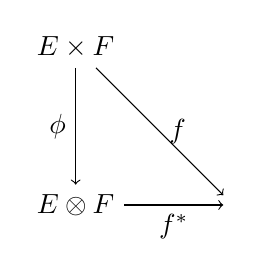
\begin{tikzpicture}
\node (EtimesF) at (0,0) {$E \times F$};
\node (EotimesF) at (0,-2) {$E \otimes F$};
\node (R) at (2,-2) {$\R$};
\draw [->] (EtimesF) edge node[left] {$\phi$} (EotimesF);
\draw [->] (EtimesF) edge node[right] {$f$} (R);
\draw [->] (EotimesF) edge node[below] {$f^*$} (R);
\end{tikzpicture}
\end{center}

Then we have,

\[ \Lin(E \otimes F, \R) \iso \Bin(E \cross F, \R) \]
\[ \Lin(f^*, \R) \iso \Bin(f, \R) \]

where `$\iso$' is used to denote \textit{isomorphic}.

\heading{Properties}

Basis for $E \otimes F$ is $e_\al \otimes g_\al$ where $e_\al$ is the basis for E and $g_\al$ is the basis for F.
For $a \in \R$ and $t, v \in E$, $u, w \in F$,

\begin{itemize}
    \item $\dim(E \otimes F) = \dim(E)\dim(F)$
    \item $a (v \otimes w) = (av) \otimes w = v \otimes (aw)$
    \item $(v + t) \otimes w = v \otimes w + t \otimes w$
    \item $v \otimes (w + u) = v \otimes w + v \otimes u$
    \item $a \otimes w = aw$
    \item $\R \otimes F = F$
\end{itemize}

Note that $V^* \otimes V^* \iso \Bin(V \times V, \R)$. To motivate this, let $f^\al \otimes f^\be$ be the basis for $V^* \otimes V^*$, and then a general element in $V^* \otimes V^*$ is,

\[ t = t_{\al\be} f^\al \otimes f^\be \]

Note that $t_{\al\be}$ is just a set of numbers. Then the tensor product is expanded as follows,

\begin{align*}
    t (v \otimes w) &= t (v^\al e_\al \otimes w^\be e_\be) \\
    &= t_{\ga\de} (f^\ga \otimes f^\de) (v^\al e_\al \otimes w^\be e_\be) \\
    &= t_{\ga\de} v^\al w^\be (f^\ga \otimes f^\de) (e_\al \otimes e_\be) \note{By linearity} \\
    &= t_{\ga\de} v^\al w^\be f^\ga(e_\al) f^\de(e_\be) \note{By foiling and definition of $f$} \\
    &= t_{\ga\de} v^\al w^\be {\delta^\ga}\al {\delta^\de}_\be \\
    &= t_{\ga\de} v^\ga w^\be {\delta^\de}_\be \note{By sifting property of $\delta$}\\
    &= t_{\ga\de} v^\ga w^\de \note{By sifting property of $\delta$ again}
\end{align*}

Since $t (v \otimes w)$ is the tensor product $V^* \otimes V^*$ and $t_{\ga\de}$ is the components of the bilinear form, one can see the connection $V^* \otimes V^* \iso \Bin(V \times V, \R)$. \\

Tensors allow one to write bilinear maps as linear maps. What about multi-linear maps?

\heading{Tensors}

A tensor of rank $\br{k,l}$ is a multi-linear map

\[ \underbrace{V^* \times \cdots \times V^*}_{k} \times \underbrace{V \times \cdots \times V}_{l} \ar \R \]

which transforms \textit{well} under the change of basis of $V$ and $V^*$. \\

\begin{center}
\label{Tensor Examples}
\begin{tabular}{c|c}
Tensor & Rank \\
\hline
vectors & $(1,0)$ \\
co-vectors & $(0,1)$ \\
scalar & $(0,0)$ \\
metric & $(0,2)$ \\
inverse metric & $(2,0)$ \\
matrix & $(1,1)$ \\
\end{tabular}
\end{center}

The set of tensors of rank $(k,l)$ is a vector space of dimension $n^{k+l}$ (if $V$ has dimension $n$). Checking with the examples above motivates this fact. \\

Using the basis $e_{\al_1} \otimes \cdots \otimes e_{\al_k} \otimes f^{\be_1} \otimes \cdots \otimes f^{\be_k}$

\[ T = {T^{\al_1\al_2\cdots\al_k}}_{\be_1\be_2\cdots\be_l} e_{\al_1} \otimes \cdots \otimes e_{\al_k} \otimes f^{\be_1} \otimes \cdots \otimes f^{\be_k}\]

For fixed $\al_i$ and $\be_i$ this is a real number in $\R$. These are the \textit{components of the tensor}. \\

By abuse of notation we will call ${T^{\al_1\al_2\cdots\al_k}}_{\be_1\be_2\cdots\be_l}$ the tensor. \\

We are talking about these transformations as change of basis of $V$ and $V^*$. Examples:
\begin{itemize}
  \item rotations (boost)
  \item change of coordinates from Cartesian to spherical, cylindrical, etc.
\end{itemize}

We can have a linear change of basis $\ti{x}^\mu = {A^\mu}_\nu x^\nu $.

\heading{Example}

\begin{center}
\begin{tabular}{c|c}
    Cartesian & Polar \\
    \hline
    $e_1 = \vec{i}$ & $\ti{e}_1 = e_r$ \\
    $e_2 = \vec{j}$ & $\ti{e}_2 = e_\theta$ \\
\end{tabular}
\end{center}

\heading{Example}

\[ \ti{e}_\al = \untext{\pder{x^\nu}{\ti{x}^\al}}{Jacobian} e_\nu = {A^{\nu}}_\al e_\nu \]

Note: \textit{Up in the denominator means down on the original coordinates (LHS).}

For example,

\begin{center}
\begin{tabular}{c|c}
    $x^1 = x$ & $\ti{x}^1 = r$ \\
    $x^2 = y$ & $\ti{x}^2 = \theta$ \\
\end{tabular}
\end{center}

\[ \ti{e}_1 = e_r = \pder{x^1}{\ti{x}^1} e_1 + \pder{x^2}{\ti{x}^1} e_2 = \cos \theta e_1 + \sin \theta e_1 \]
\[ \ti{e}_2 = e_\theta = \pder{x^1}{\ti{x}^2} e_1 + \pder{x^2}{\ti{x}^2} e_2 = - r \sin \theta e_1 + r \cos \theta e_1 \]

\heading{Vectors in multiple basis}

\[ v = v^\nu e_\nu = \ti{v}^\nu \ti{e}_\nu \]

With conversion of basis given by,

\[ \ti{e}_\al = {A^\nu}_\al e_\nu\]

Thus substituting in,

\[ v^\nu e_\nu = \ti{v}^\al {A^\nu}_\al e_\nu \note{Drop $e_\nu$}\]

\[ v^\nu = \ti{v}^\al {A^\nu}_\al \]

But with $A$ as a Jacobian,

\[ v^\nu = \pder{x^\nu}{\ti{x}^\al} \ti{v}^\al \]
\[  \ti{v}^\al = \pder{\ti{x}^\al}{x^\nu} v^\nu \]

But what about the dual space?

By definition,

\[ \ti{f}^\be\br{\ti{e}_\nu} = \delta^\be_\mu = \ti{f}^\be \br{{A^\al}_\nu e_\al} = {A^\al}_\nu \ti{f}^\be \br{ e_\al}\]

Let $\ti{f}^\be \br{ e_\al}$ be expressed as $\ti{f}^\be = {B^\be}_\ga f^\ga$

\begin{align*}
    \ti{f}^\be\br{\ti{e}_\nu} &= {A^\al}_\nu {B^\be}_\ga f^\ga \br{ e_\al} \\
    &= {A^\al}_\nu {B^\be}_\ga {\delta^\ga}_\al \\
    &= {B^\be}_\ga {A^\ga}_\nu \\
    &= {\delta^\be}_\nu
\end{align*}

Thus $B$ is the inverse of $A$. \\

What does transforming \textit{well} mean? A tensor is transforming well if its components transform as

\[{T^{\nu_1\nu_2\cdots\nu_k}}_{\al_1\al_2\cdots\al_l} \ar \pder{\ti{x}^{\nu_1}}{x^{\be_1}} \cdots \pder{\ti{x}^{\nu_k}}{x^{\be_k}} \pder{x^{\ga_1}}{\ti{x}^{\al_1}} \cdots \pder{x^{\ga_k}}{\ti{x}^{\al_k}} {T^{\be_1\be_2\cdots\be_k}}_{\ga_1\ga_2\cdots\ga_l} = {\ti{T}^{\nu_1\nu_2\cdots\nu_k}}_{\al_1\al_2\cdots\al_l} \]

If you find something like ${T^\al}_\be$, is it a tensor? \textbf{No! You must check if it transforms well.}

\[ \pder{}{x^\nu} v^\al \note{This is not a tensor.} \]

The derivative here prevents it from being well-formed. In the future we will define a derivative that allows a tensor to transform well.

\subsection{Operations on Tensors}

\begin{itemize}
    \item Add (with matching rank): ${T^{\al_1\al_2}}_{\be_1\be_2} + {C^{\al_1\al_2}}_{\be_1\be_2}$.
    \item Contraction (partial trace): $\mathcal{T} (k, k) \ar \mathcal{T} (k-1, k-1)$.
    \begin{itemize}
        \item ${T^{\al_1\cdots\al_i\cdots\al_k}}_{\be_1\cdots\be_j\cdots\be_l} \ar {T^{\al_1\cdots\al_i\cdots\al_k}}_{\be_1\cdots\al_j\cdots\be_l}$
    \end{itemize}
    \item ``Outer'' Product (Gluing together tensors)
    \begin{itemize}
        \item $\mathcal{T}(k,l) \times \mathcal{T}(k',l') \ar \mathcal{T}(k + k', l+ l')$
        \item $(T_1, T_2) \ar T_1T_2$
        \item $T_1 T_2 \ar {T_1^{\nu_1\cdots\nu_k}}_{\al_1\cdots\al_l} {T_2^{\be_1\cdots\be_k}}_{\ga_1\cdots\ga_l}$
        \item \textbf{Example:} $\br{v^\al, w_\be} \ar v^\al \otimes w_\be = v^\al w_\be$. (In QM this is $\ket{\phi}\bra{\varphi}$)
    \end{itemize}
\end{itemize}

The metric $g_{\al\be}$ can change the rank of a tensor. Recall a metric is rank $(0,2)$ is symmetric and is non-degenerate.

\heading{Example}

Changing from rank $(1,0)$ to rank $(0,1)$:

\[ v^\al \ar v_a = g_{\al\be} v^\be \]

Changing from rank $(2,2)$ to rank $(4,0)$:

\[ {C^{\al\be}}_{\ga\de} \ar C_{\al\be\ga\de} = g_{\al\rho}g_{\be\eta} {C^{\rho\eta}}_{\ga\de} \]

Changing from rank $(2,2)$ to a different rank $(2,2)$:

\[ {C^{\al\be}}_{\ga\de} \ar {{{C^{\al}}_\be}^{\ga}}_\de = g_{\be\rho}g^{\ga\eta} {C^{\al\rho}}_{\eta\de} \]

\subsection{Facts About Tensors}

\heading{Order Matters}

The order of indices that label a tensor is \textbf{very} important. It indicates the product space you are mapping \textit{from} to $\R$.
\begin{align*}
{C^\al}_\be &: \qquad V^* \times V \ar \R \\
{C_\al}^\be &: \qquad V \times V^* \ar \R \\
C_\al^\be &: \qquad \text{Nothing. Don't do this.} \\
\end{align*}

\heading{Equality between tensors}

As tensors, indices must match:\\

Position of indices is matching: ${{C^\al}_\ga}^\de = {{T^\al}_\ga}^\de$ \\

Position of indices is \textbf{not} matching: ${{C^\al}_\ga}^\de \neq {{T^\al}_\ga}_\de$ \\

But for fixed $\al, \ga, \de$, one can abuse the notation a bit:

\[ {{C^\al}_\ga}^\de = {{T^\al}_\ga}_\de \note{Try to avoid this.}\]

\subsection{Outer Product and Contraction}

\heading{Example}

Outer Product: ${M^{\al}}_\be{M^{\ga}}_\de = {{{{C^{\al}}_\be}^\ga}_\de}$ \\
Contraction: ${M^{\al}}_\be{M^{\be}}_\de = {{{{C^{\al}}_\be}^\be}_\de} = {C^\al}_\ga$

\heading{Example}

Outer product and contraction: ${C^{\al\be}}_{\ga\de}{T^{\ga\de}}_{\rho} = {A^{\al\be}}_\rho$ \\
This doesn't make sense: ${C^{\al\be}}_{\ga\ga}{T^{\ga\de}}_{\rho} = ??$ \\

Note, when there is a ``+'' sign we can be ``loose'' with the indices. Here the dual indices \textbf{do not} indicate a summation. This acts as an abuse of notation, but is sometimes difficult to avoid.

\[ C^{\al\ga}{T_\ga}^{\de} + {F_\ga}^{\de}A^{\al\ga} \]

\subsection{Interpretation of Tensors}

By looking at the indices, how can we interpret the physical meaning of the tensor object? \\

\begin{tabular}{c|l}
    Tensor & Interpretation \\
    \hline
    $v^\nu$ & vector \\
    $v_\nu$ & covector \\
    ${M^\al}_\be$ & matrix ($\al$ rows, $\be$ columns) \\
    ${M^\al}_\al$ & contracted matrix (trace) \\
    ${M^{\al\ga}}_\de$ & matrix whose elements are vectors themselves (${\cdot^\ga}_\de$ is the matrix) \\
    ${M^{\al\ga}}_\de$ & vector with matrix components (${M^\al}$ is the vector) \\
    ${R^{\al\be}}_{\ga\de}$ & matrix of matricies *\\
\end{tabular}
\vspace{0.1in}

*For example, if $\dim V = 4$, ${R^{\al\be}}_{\ga\de}$ has $4^4 = 256$ components. Note however, there can be many symmetries that reduce the number of unique components.

\subsection{Symmetry of Tensor}

We can always build a symmetric and antisymmetric part of a tensor $T^{\al\be}$. Let's look at the case of 2 indices $\al, \be$:

\heading{Symmetric Part}

\[ T_{\br{\al\be}} = \f12 \br{T_{\al\be} + T_{\be\al}} \]
\[ T_{\br{\al\be}} = T_{\br{\be\al}}  \]

\heading{Antisymmetric Part}

\[ T_{\bs{\al\be}} = \f12 \br{T_{\al\be} - T_{\be\al}} \]
\[ T_{\bs{\al\be}} = - T_{\bs{\be\al}}  \]

Note that for all tensors $T^{\al\be} = T^{\br{\al\be}} + T^{\bs{\al\be}}$. This acts as the decomposition into odd and even symmetries of the tensor. \\

For more indices:

\[ {T^{\br{\al\be}}}_{\bs{\ga\de}} = \f14\br{{T^{\al\be}}_{\ga\de} + {T^{\be\al}}_{\ga\de} - {T^{\al\be}}_{\de\ga} - {T^{\be\al}}_{\de\ga}} \]

What does $T^{\br{\al\be\ga}}$ mean? For that we will need a permutation group.

\section{Physics Review}

Moving away from tensors for a moment... \\

\subsection{Newtonian Physics}

According to Galileo and Newton, we got the interpretation that both space and time is flat $\br{\R^3}$ and is absolute. More specifically, all clocks will have the same time if they are started/synced at some shared moment. It is built on cartesian coordinate system: $\br{\vec{x}, t}$. With this we say that an object is at position $\vec{x}$ at time $t$. In this context, coordinates are \textit{outcomes of measurements}. In General Relativity, the notion of coordinates can be quite different. \\

Consider a particle (2d spacetime):

\begin{center}
\begin{tikzpicture}[scale=1.0]
    % Draw axes
    \draw [<->,thick] (0,4) node (yaxis) [above] {$x$}
        |- (5,0) node (xaxis) [right] {$t$};
    \draw [blue, thick, ->] plot [smooth, tension=1] coordinates { (0,1) (1,2) (3,1) (4,3)};
    \node [blue,above] (label) at (1,2) {$x(t)$};
\end{tikzpicture}
\end{center}

Typically, $x$ is drawn as the ordinate ($y$-axis) and $t$ as the abscissa ($x$-axis).

\heading{Spacetime diagram}

In a spacetime diagram, $t$ is drawn as the ordinate.

\begin{center}
\begin{tikzpicture}[scale=1.0]
    % Draw axes
    \draw [<->,thick] (0,4) node (yaxis) [above] {$t$}
        |- (5,0) node (xaxis) [right] {$x$};
    \draw [blue, thick, ->] plot [smooth, tension=1] coordinates { (1,0) (2,1) (1,3) (3,4)};
    \node [blue, right] (label) at (2,1) {$x(t)$};
\end{tikzpicture}
\end{center}

If we begin to use light to probe the position of objects, we are going to run into some surprising results. We will have to abandon Newtonian Physics and switch to the domain of Special Relativity.

\subsubsection{Newton's Dynamical Law \& Inertial Observers}

\[ \vec{F} = m \vec{a}\]

Where $\vec{F}$ is the total force applied to the system, $\vec{a} = \ddot{\vec{x}} = \dder{\vec{x}}{t}$ and $m$ is the inertial mass. For $\vec{x}$ is it convienent to use the Cartesian coordinate system. \\

If $\vec{F} = \vec{0}$ then the dynamics becomes $\ddot{\vec{x}} = 0$ which yields solution,

\[ \vec{x}(t) = \vec{v} t + \vec{x}_0 \]

Where $\vec{x}_0$ is the initial condition and $\vec{v}$ is the velocity in the observer's frame. This solution describes a straight line.

\begin{center}
\begin{tikzpicture}[scale=1.0]
    % Draw axes
    \draw [<->,thick] (0,4) node (yaxis) [above] {$\vec{x}$}
        |- (5,0) node (xaxis) [right] {$t$};
    \draw [blue, thick, ->] plot [smooth, tension=1] coordinates { (1,0) (3,4)};
    \node [blue, right] (label) at (2,1) {$\vec{x}(t) = \vec{v}t + \vec{x}_0$};
\end{tikzpicture}
\end{center}

However, consider this solution in a spacetime diagram,

\begin{center}
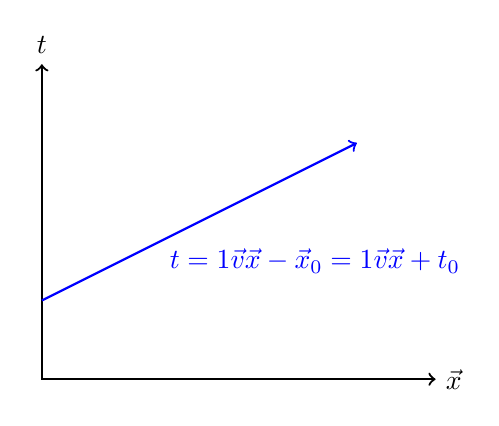
\begin{tikzpicture}[scale=1.0]
    % Draw axes
    \draw [<->,thick] (0,4) node (yaxis) [above] {$t$}
        |- (5,0) node (xaxis) [right] {$\vec{x}$};
    \draw [blue, thick, ->] plot [smooth, tension=1] coordinates { (0,1) (4,3)};
    \node [blue, right] (label) at (1.5,1.5) {$t = \f{1}{\vec{v}}\br{\vec{x} - \vec{x}_0} = \f{1}{\vec{v}}\vec{x} + t_0$};
\end{tikzpicture}
\end{center}

\heading{Definition}

The class of frames (observers) for which the the dynamics of a system is $\ddot{\vec{x}} = \vec{0}$ are called an inertial observers.

\begin{center}
\begin{tikzpicture}[scale=1.0]
    % Draw axes
    \coordinate (nya) at (0, -1);
    \coordinate (pya) at (0, 3);
    \coordinate (nxa) at (-2, 0);
    \coordinate (pxa) at (4, 0);
    \draw [<->, thick] (nya) -- (pya);
    \draw [<->, thick] (nxa) -- (pxa);
    \node [above] (lpya) at (pya) {$t$};
    \node [right] (lpxa) at (pxa) {$x$};
    \draw [orange, thick, ->] plot [smooth, tension=1] coordinates {(nya) (pya)};
    \node [orange] (label) at (-0.5, 0.5) {$x(t)$};
    \draw [red, thick, ->] plot [smooth, tension=1] coordinates {($(nya) + (1,0)$) ($(pya) + (1,0)$)};
    \node [red] (yellowlabel) at (2, 0.5) {translation};
    \draw [blue, thick, ->] plot [smooth, tension=1] coordinates {(-0.5, -1) (1.5, 3.0)};
    \node [blue, right] (label) at (1.5, 3.0) {boost};
\end{tikzpicture}
\end{center}

Note that rotations are not visible in this diagram as there is only one 1 space dimension.

Transformations that relate inertial observers:
\begin{itemize}
    \item translation: $\vec{x}(t) \ar \vec{x}'(t) = \vec{x}(t) + \vec{a}$
    \item rotation: $\vec{x}(t) \ar \vec{x}'(t) = R \cdot \vec{x}$
    \item Galilean boost: $\vec{x}(t) \ar \vec{x}'(t) = - \vec{v}t  + \vec{x}(t)$
\end{itemize}

For each of these transformations $\ddvec{x}' = \vec{0}$. We will now prove the set of all these transformation of $\vec{x}(t) \ar \vec{x}'(t)$ form a group.

\heading{Groups}

A Group is a set $G$ equipped with an associated product ($\cdot$), a unit element and an inverse.

\begin{itemize}
    \item $g_1 \cdot g_2 = g \in G, g_i \in G$
    \item $g_1 \cdot \br{g_2 \cdot g_3} = \br{g_1 \cdot g_2} \cdot g_3$
    \item $g \cdot 1 = 1 \cdot g = g$
    \item $g \cdot g^{-1} = g^{-1} \cdot g = 1$
    \item In general, $g_1 \cdot g_2 \neq g_2 \cdot g_1$.
    \item An abelian group is one where $g_1 \cdot g_2 = g_2 \cdot g_1$.
\end{itemize}

Upon careful examinations of translations and rotation of space $\R^n$, both translations and rotations form a group. What about Galilean boosts? \\

\newcommand{\wrt}{with respect to }

Consider person $A$ (Alice) standing on the ground and person $B$ (Bob) in a rocket traveling with velocity $\vec{v}_1$ \wrt $B$. Give person $B$ a ball in the rocket and let him/her kick it with velocity $\vec{v}_2$ \wrt $B$. What is the velocity of the ball \wrt person $A$? Switching between the perspectives of the system is equivalent to performing a Galilean Boost. \\

\heading{Matrix Representation of a Group}

\begin{center}
\begin{tikzpicture}[scale=1.0]
    % Draw axes
    \coordinate (nya) at (0, -1);
    \coordinate (pya) at (0, 3);
    \coordinate (nxa) at (-2, 0);
    \coordinate (pxa) at (4, 0);
    \draw [<->, thick] (nya) -- (pya);
    \draw [<->, thick] (nxa) -- (pxa);
    \node [above] (lpya) at (pya) {$t$};
    \node [right] (lpxa) at (pxa) {$x$};
    \draw [red, thick, ->] plot [smooth, tension=1] coordinates {(nya) (pya)};
    \node [red, left] (label) at (pya) {$A$};
    \draw [blue, thick, ->] plot [smooth, tension=1] coordinates {(-0.5, -1) (1.5, 3.0)};
    \node [blue, right] (label) at (1.5, 3.0) {$B$};
\end{tikzpicture}
\end{center}

The boost ${B^{\al}}_\ga$ is given by,

\[ {B^{\al}}_\ga = \mtrx{1 & 0 & 0 & 0 \\ -v_1 & 1 & 0 & 0 \\ -v_2 & 0 & 1 & 0 \\ -v_3 & 0 & 0 & 1} \]

Person $A$ (sitting on the ground) is given by,

\[ A \sim \mtrx{t \\ 0 \\ 0 \\ 0} \]

Their product is given by,

\[ \mtrx{1 & 0 & 0 & 0 \\ -v_1 & 1 & 0 & 0 \\ -v_2 & 0 & 1 & 0 \\ -v_3 & 0 & 0 & 1} \mtrx{t \\ 0 \\ 0 \\ 0} = \mtrx{t \\ -v_1t \\ -v_2t \\ -v_3t }\]

This is the trajectory of Alice \wrt Bob parametrized with time $t$. What about Bob's perspective under this linear map?

\[ \mtrx{t \\ v_1t \\ v_2t \\ v_3t } \mtrx{1 & 0 & 0 & 0 \\ -v_1 & 1 & 0 & 0 \\ -v_2 & 0 & 1 & 0 \\ -v_3 & 0 & 0 & 1} = \mtrx{t \\ -v_1t + v_1t \\ -v_2t + v_2t \\ -v_3t + v_3t \\} = \mtrx{t \\ 0 \\ 0 \\ 0} \]

Thus Galilean boosts form an abelian group. When we move to the regime of Special Relativity, we will see that boosts no longer form an abelian group.

\subsection{The Relativity Principle}

\textit{Two inertial observers moving with constant velocity cannot be distinguished by any physical experiment.} \\

Or alternatively, \\

\textit{Inertial frames are equivalent in terms of the description of physical phenomena.} \\

This is most easily observed when sitting on a train next to another train. When your train is moving, it is unclear whether or not your train is moving or the other one is. \\

Inertial frames are systems with $\ddvec{x} = \vec{0}$ equipped with rods and clocks for measurements. \\

What happens to the notion of spatial length when you change inertial frames? Nothing should change due to the Relativity Principle, the lengths should remain the same.

\begin{center}
\begin{tikzpicture}[scale=1.0]
    % Draw axes
    \coordinate (nya) at (0, -1);
    \coordinate (pya) at (0, 3);
    \coordinate (nxa) at (-2, 0);
    \coordinate (pxa) at (4, 0);
    \coordinate (xa) at (1,1.5);
    \coordinate (xb) at (3,1.5);
    \draw [<->, thick] (nya) -- (pya);
    \draw [<->, thick] (nxa) -- (pxa);
    \node [above] (lpya) at (pya) {$t$};
    \node [right] (lpxa) at (pxa) {$x$};
    \draw [red, thick] plot [smooth, tension=1] coordinates {(xa) (xb)};
    \fill [red] (xa) circle (1pt) node[left] {$x_A$};
    \fill [red] (xb) circle (1pt) node[right] {$x_B$};
\end{tikzpicture}
\end{center}

In one frame,
\[ \abs{\vec{x}_B - \vec{x}_A }^2 = \ell^2 \]

Perform a Galilean boost,

\[ \vec{x}'_{A,B} = -\vec{v}t + \vec{x}_{A,B} \]
\[ \abs{\vec{x}'_B - \vec{x}'_A }^2 = \ell'^2 \]
But it must be that,

\[ \ell' = \ell \]

What about time? Galilean transformation leave time invariant because time is absolute in this Newtonian regime. The notion of simultaneity is the same for any inertial observer.


\begin{center}
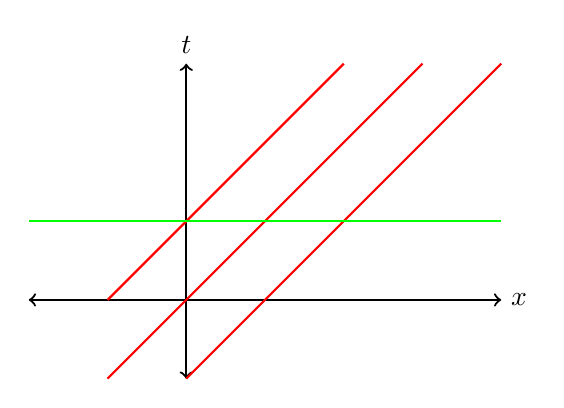
\begin{tikzpicture}[scale=1.0]
    % Draw axes
    \coordinate (nya) at (0, -1);
    \coordinate (pya) at (0, 3);
    \coordinate (nxa) at (-2, 0);
    \coordinate (pxa) at (4, 0);
    \draw [<->, thick] (nya) -- (pya);
    \draw [<->, thick] (nxa) -- (pxa);
    \node [above] (lpya) at (pya) {$t$};
    \node [right] (lpxa) at (pxa) {$x$};
    \draw [red, thick] plot [smooth, tension=1] coordinates {(-1,-1) (3,3)};
    \draw [red, thick] plot [smooth, tension=1] coordinates {(-1,0) (2,3)};
    \draw [red, thick] plot [smooth, tension=1] coordinates {(0,-1) (4,3)};
    \draw [green, thick] plot [smooth, tension=1] coordinates {(-2,1) (4,1)};
\end{tikzpicture}
\end{center}

Red lines are stationary observers, and intersection with red lines indicate simultaneous events.

\heading{Math Perspective}

Are Galilean transformations the most general transformations between inertial observers? Use axioms?

\heading{Physics Perspective}

\begin{itemize}
    \item Maxwell's equations do not transform well under Galilean transforms. Lorentz found the Lorentz transformations that allow Maxwell's equations to transform well.
    \item Michelson-Morley experiment: reveals that speed of light is invariant under the change of frame.
    \begin{itemize}
        \item $v_1 + v_2 = v_3$ This is \textbf{not} the case if $v_2 = c$
        \item $v_1 + c = c$ What why???
        \item Under the assumption that light is a wave in the ether. Results suggest that the ether is not measurable.
    \end{itemize}
\end{itemize}

\subsection{Lorentz Transformations}

Let's use light to measure objects in two frames; specifically let's determine the position using light.

\heading{Assumptions}

\begin{itemize}
    \item The speed of light is the same in any frame.
    \item Relativity Principle
    \item Bob will move at velocity $v < c$
    \begin{itemize}
        \item If an observer is moving $v > c$, their position can't be measured using light
    \end{itemize}
    \item 2d for simplicity
    \item Set $c=1$, $x=ct + x_0 = t + x_0$
\end{itemize}

\begin{center}
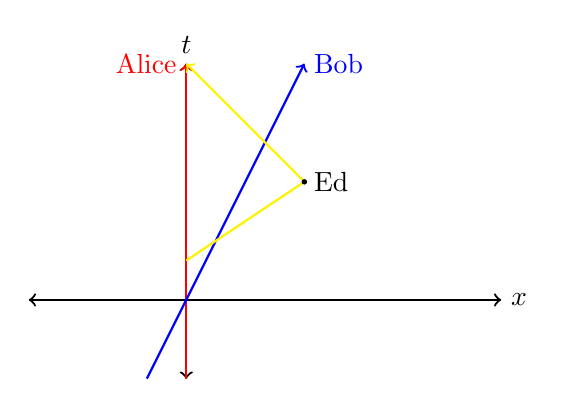
\begin{tikzpicture}[scale=1.0]
    % Draw axes
    \coordinate (nya) at (0, -1);
    \coordinate (pya) at (0, 3);
    \coordinate (nxa) at (-2, 0);
    \coordinate (pxa) at (4, 0);
    \coordinate (ed) at (1.5, 1.5);
    \node [above] (lpya) at (pya) {$t$};
    \node [right] (lpxa) at (pxa) {$x$};
    \draw [<->, thick] (nya) -- (pya);
    \draw [<->, thick] (nxa) -- (pxa);
    \draw [->, thick, red] (nya) -- (pya);
    \draw [->, thick, blue] (-0.5, -1) -- (1.5,3);
    \draw [->, thick, yellow] (0, 0.5) -- (ed) -- (pya);
    \node [left, red] (alicelabel) at (pya) {Alice};
    \node [right, blue] (boblabel) at (1.5,3) {Bob};
    \node [right] (edlabel) at (ed) {Ed};
    \fill (ed) circle[radius=1pt];
\end{tikzpicture}
\end{center}

Let's measure the coordinates of Ed in Alice's frame and Bob's frame and the map relating the times using light to measure positions.

1) Using light to measure position,

\[ x = \f{1}{2c}\br{t_2 - t_1} \]
\[ T = t_1 + \f12 \br{t_2 - t_1} = \f12 \br{t_2 + t_1} \]

\begin{center}
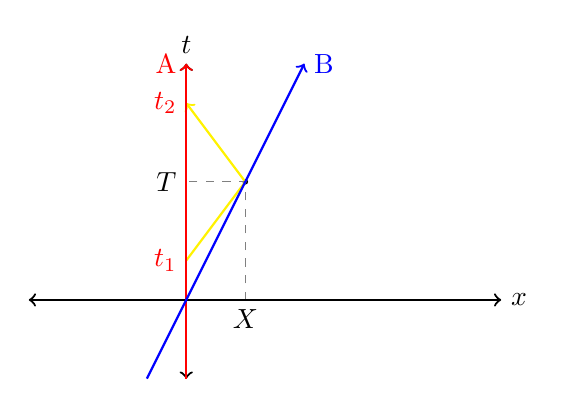
\begin{tikzpicture}[scale=1.0]
    % Draw axes
    \coordinate (nya) at (0, -1);
    \coordinate (pya) at (0, 3);
    \coordinate (nxa) at (-2, 0);
    \coordinate (pxa) at (4, 0);
    \node [above] (lpya) at (pya) {$t$};
    \node [right] (lpxa) at (pxa) {$x$};
    \coordinate (xt) at (0.75, 1.5);
    \coordinate (X) at (0.75, 0);
    \coordinate (T) at (0, 1.5);
    \coordinate (t1) at (0, 0.5);
    \coordinate (t2) at (0, 2.5);
    \node [left, red] (t1label) at (t1) {$t_1$};
    \node [left, red] (t1label) at (t2) {$t_2$};
    \node [left] (Tlabel) at (T) {$T$};
    \node [below] (Xlabel) at (X) {$X$};
    \fill (xt) circle[radius=1pt];
    \draw [->, thick, yellow] (t1) -- (xt) -- (t2);
    \draw [dashed, gray] (X) -- (xt) -- (T);
    \draw [<->, thick] (nya) -- (pya);
    \draw [<->, thick] (nxa) -- (pxa);
    \draw [->, thick, red] (nya) -- (pya);
    \draw [->, thick, blue] (-0.5, -1) -- (1.5,3);
    \node [left, red] (alicelabel) at (pya) {A};
    \node [right, blue] (boblabel) at (1.5,3) {B};
\end{tikzpicture}
\end{center}

2) Determine how the difference of times of reception and emission are related?

\[ \De t_A = ON \quad \De t_B = QP \]
\[ \f{MN}{OM} = \f{MP}{QM} \]
\[ \f{MN}{MN+\Delta t_A} = \f{MP}{MP+\Delta t_B} \]
\[ \f{\Delta t_A}{MN} = \f{\Delta t_B}{MP} \]
\[ \Delta t_A \propto \Delta t_B \]

\begin{center}
\begin{tikzpicture}[scale=1.5]
    % Draw axes
    \coordinate (nya) at (0, -1);
    \coordinate (pya) at (0, 3);
    \coordinate (nxa) at (-2, 0);
    \coordinate (pxa) at (4, 0);
    \draw [<->, thick] (nxa) -- (pxa);
    \draw [<->, thick] (nya) -- (pya);
    \node [above] (lpya) at (pya) {$t$};
    \node [right] (lpxa) at (pxa) {$x$};
    \coordinate (ai) at (nya);
    \coordinate (bi) at (-0.2, -1);
    \coordinate (af) at (pya);
    \coordinate (bf) at (1.8, 3);
    \draw [->, thick, red] (ai) -- (af);
    \draw [->, thick, blue] (bi) -- (bf);
    \node [left, red] (la) at (af) {A};
    \node [right, blue] (lb) at (bf) {B};
    \coordinate (lt0) at (intersection of nya--pya and bi--bf);
    \coordinate (lx0) at (intersection of nxa--pxa and bi--bf);

    \coordinate (M) at (lt0);
    \coordinate (O) at (0, 1.5);
    \coordinate (N) at (0, 1);
    \coordinate (P) at (intersection of O--(3,2.5) and bi--bf);
    \coordinate (Q) at (intersection of N--(3,2) and bi--bf);

    \draw [->, thick, yellow] (N) -- (Q);
    \draw [->, thick, yellow] (O) -- (P);

    \fill (lx0) circle (1pt) node[below right] {$x_0$};
    \fill (lt0) circle (1pt) node[left] {$t_0$};
    \fill (Q) circle (1pt) node[right] {$Q$};
    \fill (O) circle (1pt) node[right] {$O$};
    \fill (N) circle (1pt) node[right] {$N$};
    \fill (M) circle (1pt) node[right] {$M$};
    \fill (P) circle (1pt) node[right] {$P$};
\end{tikzpicture}
\end{center}

\[ \Delta t_A = f^{-1}(v, c, x_0, y_0) \Delta t_B \]

By translational invariance, $f$ cannot depend on $x_0$ or $t_0$. Therefore,

\[ \Delta t_A = f^{-1}(v, c) \Delta t_B \]

For convenience, we will find $f$ defined as,

\[ \Delta t_B = f(v, c) \Delta t_A \]

By similar analysis of a pair of light rays emanating from bob,

\[ \Delta \ti{t}_A = \ti{f}(v, \ti{c}) \Delta \ti{t}_B = \ti{f}(v, c) \Delta \ti{t}_B \]

This uses the assumption $\ti{c} = c$. Furthermore by the relativity principle, we must have $\ti{f} = f$. Otherwise, the two inertial frames ($A, B$) would be distinguishable through $f, \ti{f}$. In conclusion:

\[ \De t\tsb{received} = f(v,c) \De t\tsb{emitted} \]

So what is the form of $f$? Let us assume that there is a synchronization between the two frames so that calculations become easier.

\begin{center}
\begin{tikzpicture}[scale=1.5]
    % Draw axes
    \coordinate (nya) at (0, -1);
    \coordinate (pya) at (0, 3);
    \coordinate (nxa) at (-2, 0);
    \coordinate (pxa) at (4, 0);
    \draw [<->, thick] (nxa) -- (pxa);
    \draw [<->, thick] (nya) -- (pya);
    \node [above] (lpya) at (pya) {$t$};
    \node [right] (lpxa) at (pxa) {$x$};
    \coordinate (ai) at (nya);
    \coordinate (bi) at (-0.33, -1);
    \coordinate (af) at (pya);
    \coordinate (bf) at (1, 3);
    \draw [->, thick, red] (ai) -- (af);
    \draw [->, thick, blue] (bi) -- (bf);
    \node [left, red] (la) at (af) {A};
    \node [right, blue] (lb) at (bf) {B};

    \coordinate (t0) at (0, 1);
    \coordinate (tau) at (intersection of t0--(3,4) and bi--bf);
    \coordinate (tL) at ($(tau) + (0, -10)$);
    \coordinate (tT) at ($(tau) + (-10, 0)$);
    \coordinate (L) at (intersection of tau--tL and nxa--pxa);
    \coordinate (T) at (intersection of tau--tT and nya--pya);
    \coordinate (t1) at (intersection of tau--(-3,5) and ai--af);

    \draw [->, thick, yellow] (t0) -- (tau);
    \draw [->, thick, yellow] (tau) -- (t1);
    \draw [dashed, gray] (tau) -- (L);
    \draw [dashed, gray] (tau) -- (T);

    \fill (t0) circle (1pt) node[left] {$t_0$};
    \fill (tau) circle (1pt) node[right] {$\tau$};
    \fill (t1) circle (1pt) node[left] {$t_1$};
    \fill (0,0) circle (1pt) node[below right] {$S$};
    \fill (T) circle (1pt) node[left] {$T$};
    \fill (L) circle (1pt) node[below] {$L$};
\end{tikzpicture}
\end{center}

Let's define:
\begin{align*}
    \De t_A &= S \ar t_0 = t_0 \\
    \De \ti{t}_A &= S \ar t_1 = t_1 \\
    \De t_B &= S \ar \tau = \tau = \De \ti{t}_B \\
\end{align*}

Therefore $\tau = f(v,c) t_0$ with,

\[ t_1 = \De \ti{t}_A = f(v,c) \De \ti{t}_B = f^2(v,c) t_0 \]
Thus we have from radar measurements,

\[ L = \f12 c \br{t_1 - t_0} = \f12 c\br{f^2(v,c) - 1}t_0 \]
\[ T = \f12 \br{t_1 + t_0} = \f12 c\br{f^2(v,c) + 1}t_0 \]

The ratio is given by,

\[ \f{L}{T} = v = c \f{f^2(v,c) -1}{f^2(v,c) +1} \]

Inverting this expression (using $-c < v < c$) yields,

\[ f(v,c) = \br{\f{1+\f{v}{c}}{1 - \f{v}{c}}}^{1/2} \]

4) Ed's coordinate from A's and B's perspective.


\begin{center}
\begin{tikzpicture}[scale=1.5]
    % Draw axes
    \coordinate (nya) at (0, -1);
    \coordinate (pya) at (0, 3);
    \coordinate (nxa) at (-2, 0);
    \coordinate (pxa) at (4, 0);
    \draw [<->, thick] (nxa) -- (pxa);
    \draw [<->, thick] (nya) -- (pya);
    \node [above] (lpya) at (pya) {$t$};
    \node [right] (lpxa) at (pxa) {$x$};
    \coordinate (ai) at (nya);
    \coordinate (bi) at (-0.33, -1);
    \coordinate (af) at (pya);
    \coordinate (bf) at (1, 3);
    \coordinate (e) at (1, 1.5);
    \draw [->, thick, red] (ai) -- (af);
    \draw [->, thick, blue] (bi) -- (bf);
    \node [left, red] (la) at (af) {A};
    \node [right, blue] (lb) at (bf) {B};

    \coordinate (t1a) at (0, 1);
    \coordinate (t2a) at (0, 2);
    \coordinate (t1b) at (intersection of t1a--e and bi--bf);
    \coordinate (t2b) at (intersection of t2a--e and bi--bf);

    \draw [->, thick, yellow] (t1a) -- (e);
    \draw [->, thick, yellow] (e) -- (t2a);

    \fill (t1a) circle (1pt) node[left] {$T_1^A$};
    \fill (t2a) circle (1pt) node[left] {$T_2^A$};
    \fill (t1b) circle (1pt) node[right] {$T_1^B$};
    \fill (t2b) circle (1pt) node[right] {$T_2^B$};
    \fill (0,0) circle (1pt) node[below right] {$S$};
    \fill (e) circle (1pt) node[right] {$E$};
\end{tikzpicture}
\end{center}

Let $E$ be identified in two ways,
\begin{center}
\begin{tabular}{c|c}
    Alice's Perspective & $(x_A^E, t_A^E)$ \\
    \hline
    Bob's Perspective & $(x_B^E, t_B^E)$ \\
\end{tabular}
\end{center}

Therefore,
\[ x_A^E = \f12 c \br{T_2^A - T_1^A} \]
\[ t_A^E = \f12 \br{T_2^A + T_1^A} \]
\[ x_B^E = \f12 c \br{T_2^B - T_1^B} \]
\[ t_B^E = \f12 \br{T_2^B + T_1^B} \]

We know that $T_1^B = f T_1^A$ and $T_2^A = f T_2^B$ hence we can get the relation between $(x_A^E, t_A^E)$ and $(x_B^E, t_B^E)$.

\[ x_B^E = \f{1}{\sqrt{1 - \f{v^2}{c^2}}} \br{x_A^E - vt_A^E} \]
\[ t_B^E = \f{1}{\sqrt{1 - \f{v^2}{c^2}}} \br{t_A^E - \f{v}{c^2}x_A^E} \]

For convenience we can relabel,
\[ \ga =  \f{1}{\sqrt{1 - \f{v^2}{c^2}}} \]

In matrix form,
\[ \mtrx{T' \\ X'} = \underbrace{\ga \mtrx{1 & \f{-v}{c^2} \\ -v & 1}}_{\text{Lorentz Boost}} \mtrx{T \\ X}\]

Notice in the limit that $v << c$, the Lorentz boost becomes equivalent to the Galilean boost discussed earlier.

\subsubsection{Consequences of Lorentz Transformations}

\begin{enumerate}
    \item From Alice's perspective, Bob's time axis is,
    \begin{itemize}
        \item $x^B = 0 = \ga (x_A - vt_A) \implies x = vt$
    \end{itemize}
    \item From Alice's perspective, Bob's spatial slice is,
    \begin{itemize}
        \item $T^B = 0 = \ga \br{t_A - \f{v}{c^2}} x_A \implies t = \f{v}{c^2} x$
        \item The slope of this line in Alice's perspective is the \textbf{inverse} (with $c \ar 1$) of the slope of Bob's time axis
    \end{itemize}
\end{enumerate}

Again, notice that Galilean simultaneity is recovered in the limit that $v \ar v \ll c$. Our new theory is still consistent with our old theories.

\subsection{Length \& Time}

\subsubsection{Einstein's Train \& Simultaneity}
\begin{center}
\begin{tikzpicture}
    \coordinate (b) at (-3, 0);
    \coordinate (r) at (3, 0);
    \coordinate (v) at (0, 1);
    \coordinate (v2) at (1, 1);
    \coordinate (s) at (0, -1);

    \draw [->, thick] (v) -- (v2);
    \draw [dashed, gray, thick] (b) -- (r);

    \fill [blue] (b) circle (3pt) node[left] {Blue Light};
    \fill [red] (r) circle (3pt) node[right] {Red Light};
    \fill (v) circle (1pt) node[above right] {$v$};
    \fill (v) circle (1pt) node[above left] {Alice};
    \fill (s) circle (1pt) node[below] {Bob};
\end{tikzpicture}
\end{center}


\begin{center}
\begin{tikzpicture}[scale=1.5]
    % Draw axes
    \coordinate (nya) at (0, -1);
    \coordinate (pya) at (0, 3);
    \coordinate (nxa) at (-2, 0);
    \coordinate (pxa) at (4, 0);
    \draw [<->, thick] (nxa) -- (pxa);
    \draw [<->, thick] (nya) -- (pya);
    \node [above] (lpya) at (pya) {$t$};
    \node [right] (lpxa) at (pxa) {$x$};
    \coordinate (ai) at (nya);
    \coordinate (af) at (pya);
    \coordinate (bi) at (-0.33, -1);
    \coordinate (bf) at (1, 3);
    \coordinate (l1) at (-1.5, 0);
    \coordinate (l2) at (1.5, 0);
    \coordinate (lightleft) at (-5, 5);
    \coordinate (lightright) at (5, 5);
    \coordinate (l1l) at ($(l1) + (lightleft)$);
    \coordinate (l1r) at ($(l1) + (lightright)$);
    \coordinate (l2l) at ($(l2) + (lightleft)$);
    \coordinate (l2r) at ($(l2) + (lightright)$);

    \coordinate (l1i) at (intersection of bi--bf and l1--l1r);
    \coordinate (l2i) at (intersection of ai--af and l2--l2l);
    \coordinate (l1ii) at (intersection of bi--bf and l2--l2l);

    \draw [->, thick, red] (ai) -- (af);
    \draw [->, thick, yellow] (l1) -- (l1i);
    \draw [->, thick, yellow] (l2) -- (l2i);
    \draw [->, thick, blue] (bi) -- (bf);
    \node [left, red] (la) at (af) {A};
    \node [right, blue] (lb) at (bf) {B};

    \fill (l1) circle (1pt);
    \fill (l2) circle (1pt);
    \fill (l2i) circle (1pt);
    \fill (l1i) circle (1pt);
    \fill (l1ii) circle (1pt);
\end{tikzpicture}
\end{center}

Therefore, simultaneity is \textbf{relative}.

\subsubsection{Length}

What about spatial length? Alice has a ruler of length $x_2 - x_1 = \ell$. In Bob's frame,

\[ x_i = \br{\untext{x'_i + v t'}{Bob's coords}} \ga \quad i = 1,2 \]

Thus,

\[ x'_2 - x'_1 = \br{x_2 - x_1} \f{1}{\ga} \implies \ell' = \f{\ell}{\ga} \note{Length contraction.}\]

If Bob has a ruler of length $\ell' = x'_2 - x'_1$,

\[ x'_i = \br{\untext{x_i + v t}{Alice's coords}} \ga \quad i = 1,2 \]

\[ x_2 - x_1 = \ell = \f{1}{\ga}\ell'\note{Length contraction.}\]

\subsubsection{Time}

In a similar manner, we have time dilation,

\[ t'_2 - t'_1 = \ga \br{t_2 - t_1} \note{With $\ga > 1$.} \]

\subsubsection{Invariant Length \& Minkowski Metric}

Can we construct/define a notion of length that is invariant under these transformations? Namely,

\newcommand{\Lam}{\Lambda}

\[ \mtrx{\ga & -\ga \f{v}{c^2} \\ -\ga v & \ga} = {\Lam^{\al}}_{\be} \]

Let's introduce a metric, $g_{\al\be}$ that is of course symmetric and non non-degenerate. Therefore,

\[ {\Lam^{\al}}_{\be} g_{\al\ga} {\Lam^{\ga}}_{\de} = g_{\be\de}  \]

Reminder: $v \cdot w = v' \cdot w'$ with $v'^\al = {\Lam^{\al}}_{\ga} v^\ga$. The solution here for 1d motion:

\[ g_{\al\be} = \mtrx{-1 & 0 \\ 0 & 1} \text{ or } \mtrx{1 & 0 \\ 0 & -1} \]

These are called \textit{Minkowski Metrics}. The difference between these two is a matter of convention. We will select the convention,

\[ g_{\al\be} = \mtrx{-1 & 0 \\ 0 & 1}\]

\begin{center}
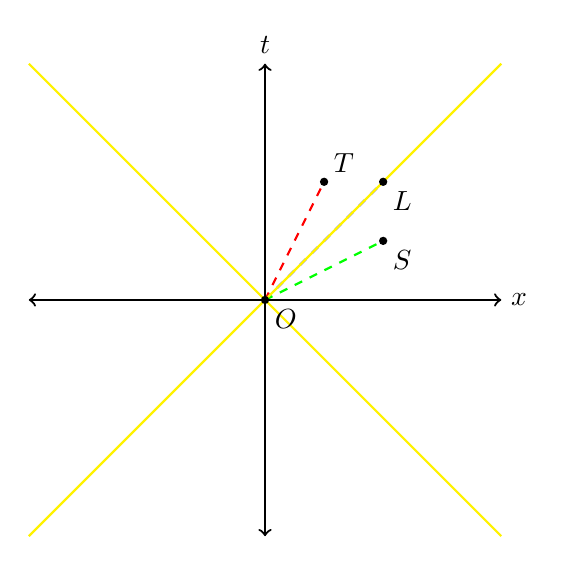
\begin{tikzpicture}[scale=1.5]
    % Draw axes
    \coordinate (nya) at (0, -2);
    \coordinate (pya) at (0, 2);
    \coordinate (nxa) at (-2, 0);
    \coordinate (pxa) at (2, 0);
    \draw [<->, thick] (nxa) -- (pxa);
    \draw [<->, thick] (nya) -- (pya);
    \node [above] (lpya) at (pya) {$t$};
    \node [right] (lpxa) at (pxa) {$x$};
    \coordinate (o) at (0,0);
    \coordinate (T) at (0.5,1);
    \coordinate (L) at (1,1);
    \coordinate (S) at (1,0.5);

    \draw [dashed, thick, red] (o) -- (T);
    \draw [dashed, thick, blue] (o) -- (L);
    \draw [dashed, thick, green] (o) -- (S);
    \draw [thick, yellow] (-2,-2) -- (2,2);
    \draw [thick, yellow] (-2,2) -- (2,-2);

    \fill (T) circle (1pt) node[above right] {$T$};
    \fill (o) circle (1pt) node[below right] {$O$};
    \fill (S) circle (1pt) node[below right] {$S$};
    \fill (L) circle (1pt) node[below right] {$L$};
\end{tikzpicture}
\end{center}

Let us define,

\begin{align*}
\abs{\vec{OT}}^2 &< 0 \note{``time like''} \\
\abs{\vec{OL}}^2 &= 0 \note{``light like''} \\
\abs{\vec{OS}}^2 &> 0 \note{``space like''}
\end{align*}

We say that a vector $v^\al$ is time-like if $v^\al \eta_{\al\be} v^\be \defined \abs{v}^2 < 0$, light-like if $v^\al \eta_{\al\be} v^\be \defined \abs{v}^2 = 0$ and space-like if $v^\al \eta_{\al\be} v^\be \defined \abs{v}^2 > 0$. \\

What are inertial observers in the relativistic regime? They are \textit{still} given by a \textit{straight lines}. What are the set of transformations relating inertial observers (4d) ?

\begin{itemize}
    \item rotations: $R_x, R_y, R_z$
\end{itemize}

\[ \ar \mtrx{1 & 0 & 0 & 0 \\ 1 & \cos \theta & \sin \theta & 0 \\ 0 & -\sin \theta & \cos \theta & 0 \\ 0 & 0 & 0 & 1 } \]

\begin{itemize}
    \item boost: $B_x, B_y, B_z$
\end{itemize}

\[ B_z \ar \mtrx{\ga & -\ga\f{v}{c^2} & 0 & 0 \\ -\ga v & \ga & 0 & 0 \\ 0 & 0 & 1 & 0 \\ 0 & 0 & 0 & 1 } \]

Therefore,

\[ \det B_z = \ga^2 - \ga^2 \f{v^2}{c^2} = \ga^2\br{1-\f{v^2}{c^2}} = 1 \]

Let us relabel $\ga^2 = \cosh^2 \eta$ and $\ga^2\f{v^2}{c^2} = \sinh^2 \eta$,

\[ B_z \ar \mtrx{\cosh \eta & -\f{\sinh \eta}{c^2} & 0 & 0 \\ -\sinh \eta & \cosh \eta & 0 & 0 \\ 0 & 0 & 1 & 0 \\ 0 & 0 & 0 & 1 } \]

\begin{itemize}
    \item translation: $\vec{x} \ar \vec{x} + \vec{a}$; $t \ar t + b$
    \begin{itemize}
        \item $x^\nu \ar x^\nu + a^\nu$
    \end{itemize}
\end{itemize}

All of these together form the Poincaré group.

\subsubsection{Poincaré Group}

Galilean boosts:

\[ \vec{v}_1 + \vec{v}_2 = \vec{v}_3 \]

Lorentzian boosts:

\[ \ovec{v_1 \oplus v_2} = \f{1}{1+\f{\vec{v}_1\cdot\vec{v}_2}{c^2}}\br{\vec{v}_1 + \f{1}{\ga_1}\vec{v}_2 + \f{1}{c}\f{\ga_1}{1-\ga_1}\br{\vec{v}_1\cdot\vec{v}_2} \vec{v}_2}\]

Note these aren't associative,

\[ \ovec{\ovec{v_1 \oplus v_2} \oplus v_3} \neq \ovec{v_1 \oplus \ovec{v_2 \oplus v_3}} \]

However it $\vec{v}_1$ is parallel to $\vec{v}_2$ then,

\[ \ovec{v_1 \oplus v_2} = \f{\vec{v}_1 + \vec{v}_2}{1 + \f{\vec{v}_1 \cdot \vec{v}_2}{c^2}} \]

Which forces $\abs{\ovec{v_1 \oplus v_2}}^2 = c^2$ whenever either $\vec{v}_1$ or $\vec{v}_2$ has $\abs{\vec{v}_i}^2 = c^2$.

\section{Formulation of Gravity}

\subsection{Flat Spacetime}

Spacetime is $\R^4$ and we will consider the Minkowski metric $\eta_{\al\be}$. In Cartesian coordinates,
\[ x^\mu = \mtrx{ct& x & y & z} \]

Consider a curve in spacetime $x^\nu(\ell)$ where $\ell$ is a curvilinear parameter that parametrizes the curve. The tangent vector is given by $\der{x^\mu}{\ell}$.

\begin{center}
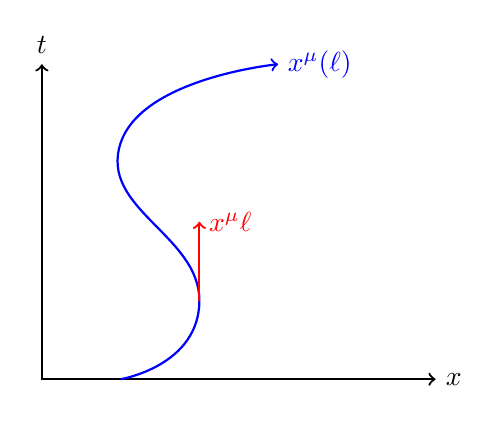
\begin{tikzpicture}[scale=1.0]
    % Draw axes
    \draw [<->,thick] (0,4) node (yaxis) [above] {$t$}
        |- (5,0) node (xaxis) [right] {$x$};
    \draw [blue, thick, ->] plot [smooth, tension=1] coordinates { (1,0) (2,1) (1,3) (3,4)};
    \draw [red, thick, ->] plot [smooth, tension=1] coordinates { (2,1) (2,2)};
    \node [blue, right] (label) at (3,4) {$x^\mu(\ell)$};
    \node [red, right] (label) at (2,2) {$\der{x^\mu}{\ell}$};
\end{tikzpicture}
\end{center}

If the tangent $\der{x^\mu}{\ell}$ is always time-like, then the curve is called time-like. Analogously for space-like and light-like curves. We can then define an arclength of the curve.

\[ \tau \neq \intl \sqrt{\der{x^\mu}{\ell} n_{\mu\nu} \der{x^\nu}{\ell}} \dif \ell \]

This expression does not work because the metric $\eta_{\mu\nu}$ is not positive definite. Therefore the length could be complex. To combat this, introduce an absolute magnitude,

\[ \tau = \intl \sqrt{\abs{\der{x^\mu}{\ell} n_{\mu\nu} \der{x^\nu}{\ell}}} \dif \ell \]

Which suggests,
\[ \der{\tau}{\ell} = \sqrt{\abs{\der{x^\mu}{\ell} n_{\mu\nu} \der{x^\nu}{\ell}}} \]
Which implies
\[ \dif \tau ^2 = \abs{\dif x^\mu n_{\mu\nu} \dif x^\nu} \]

Now consider using $\tau$ as the curvilinear parameter. So that the tangent is defined as,

\[ \der{x^\mu}{\tau} \]

What does this encapsulate? Consider an observer at rest:

\begin{center}
\begin{tikzpicture}
    % Draw axes
    \coordinate (nya) at (0, -1);
    \coordinate (pya) at (0, 3);
    \coordinate (nxa) at (-1, 0);
    \coordinate (pxa) at (3, 0);
    \draw [<->, thick] (nxa) -- (pxa);
    \draw [<->, thick] (nya) -- (pya);
    \node [above] (lpya) at (pya) {$t$};
    \node [right] (lpxa) at (pxa) {$x$};

    \draw [->, thick, blue] (nya) -- (pya);
    \draw [->, thick, red] (0,0.2) -- (0,1.0);
    \node [red, right] (label) at (0,1) {$\der{x^\mu}{\tau}$};
    \node [blue, right] (lpya2) at (pya) {$x^\mu(\ell)$};

\end{tikzpicture}
\end{center}

Here, the notion of arclength coincides with time.

\[ \dif \tau^2 = \dif t^2 \]

Considering a time-like curve, the proper length or arclength is interpreted as the time as measured by a clock carried by the observer having the curve as his/her spacetime trajectory (world-line). \\

Parametrization of the world line of an observer at rest $(\vec{x} = \vec{0})$.
\[ x^0(\tau) = \tau \quad \text{ and } \quad \vec{x} = \vec{0} \]
Which gives,
\[ \der{x^\mu}{\tau} = \mtrx{1 \\ 0 \\ 0 \\ 0} = {\de^\mu}_0 \neq {\de^0}_\mu \note{Be careful to matching indices.} \]
Labeling ${\de^\mu}_0 = V^\al$,
\[ V^\al \eta_{\al\be} V^\be = {\de^\al}_0 \eta_{\al\be} {\de^\be}_0 = \eta_{00}= -1 < 0  \]
Therefore, $V^\al$ is time-like. However in general,

\begin{align*}
V^\mu \eta_{\mu\be} V^\be &= \der{x^\mu}{\tau}  \eta_{\mu\al} \der{x^\al}{\tau}\\
&= \f{\dif x^\mu\eta_{\mu\al} \dif x^\al}{\dif \tau^2}\\
&= \f{\dif s^2}{\dif \tau^2} \note{$\ds^2$ is the line element.}\\
&= -1 \note{Since $\dif \tau^2 = \abs{\dif s^2} = - \dif s^2 $ (this vector is time-like).}\\
\end{align*}

We can can also write (with $c=1$),
\begin{align*}
\dif \tau^2 &= \dif t^2 - \dif \vec{x}^2 \\
&= \dif t^2\br{1 - \f{\dif \vec{x}^2}{\dif t^2}} \\
&= \dif t^2\br{1 - \vec{v}^2} \\
\end{align*}
Which when rearranged yields (noting the negative is ignored because we are considering time moving forward),
\[ \der{t}{\tau} = \f{1}{\sqrt{1-\vec{v}^2}} = \ga \]

Noting that,
\[ v^\mu = \mtrx{\der{t}{\tau} c \\ \der{\vec{x}}{\tau}} = \mtrx{\ga c \\ \der{t}{\tau}\der{\vec{x}}{t}} = \mtrx{\ga c \\ \ga\vec{v}} \]

Noting that $\vec{v}$ is a velocity in 3d space while $v^\mu$ is a relativistic velocity which is a 4d object. We have shown that,

\[ v^\mu v_\mu = -1 \]

In the Galilean regime, $\vec{v} \in \R^3$ which allows one to use the vector space structure of $\R^3$ to add velocities,

\[ \vec{v}_1 + \vec{v}_2 = \vec{v}_{12}\]

But for relativistic velocities $\vec{v} \in \mathbb{H}^3$ hyperboloid.

\[ \bc{v^\mu \in \R^4 \mid v^\mu v_\mu = -1} \]

This is somewhat surprising, bur there exists a constraint that reduces the dimensionality.

\[ v^\mu v_\mu = -1 = - \br{v^t}^2 + \br{v^x}^2 + \br{v^y}^2 + \br{v^z}^2 \]

\begin{center}
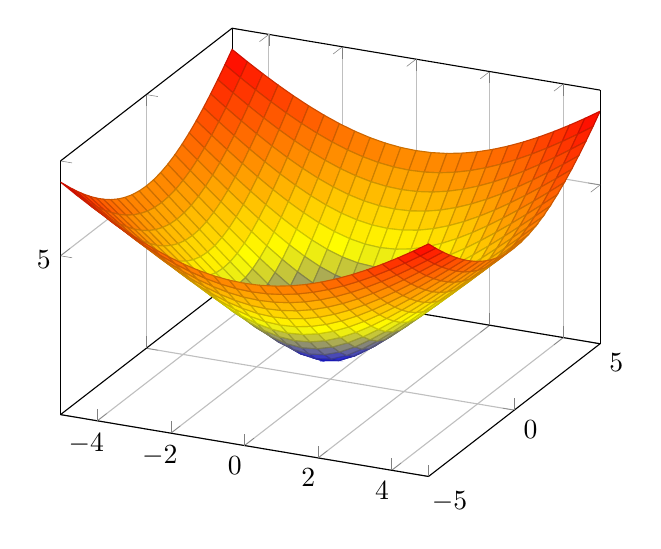
\begin{tikzpicture}
\begin{axis}[grid=both]
\addplot3[surf,shader=faceted] {sqrt(x^2 + y^2 + 1)};
\end{axis}
\end{tikzpicture}
\end{center}

This new space $\mathbb{H}^3$ allows for the addition of velocities,

\[ \ovec{v_1 \oplus v_2} = \vec{v}_{12} \]

\heading{Particle Considerations}

\begin{itemize}
    \item The world-line of a material particle is a time-like curve
    \item The world-line of photons (massless) is a light-like curve
    \item The world-line of a tachyon ($\abs{v} > c$) is space-like
\end{itemize}

Relativistic acceleration is given by,
\[ a^\mu = \der{v^\mu}{\tau} = \dder{x^\mu}{\tau} \]

For inertial observer, $a^\mu = 0$.

Relativistic momentum is given for a material particle with mass $m$,

\[ p^\mu = m v^\mu \implies p^\mu p_\mu = - m^2\]

Which has the property,

\[ p^\mu = \mtrx{E = m \ga \\ \vec{p} = m\ga \vec{v}} \]

Examine the space term,

\[ E = m \ga = m \f{1}{\sqrt{1-v^2}} = m + \untext{\f12 m v^2}{kinetic energy} + \cdots \note{Taylor Series} \]

And also rest,

\[ E^2 = m^2 c^4 \]

\subsection{Relativistic Dynamics}

What about the dynamics in the relativistic regime? Recall in the non-relativistic regime, Newton's law is given by,

\[ m_i \vec{a} = \vec{F}\tsb{tot} \]

Where $m_i$ is the inertial mass. How can we modify this equation to the relativistic regime. $m_i$ has no need to change, $\vec{a}$ becomes the 4d spacetime vector $a^\mu = \dder{x^\nu}{\tau}$ and force becomes,
\[ m_i a^\mu = F^\mu \]

\subsubsection{Lorentz Force}

Consider the Lorentz force,
\[ \vec{F} = q \br{\vec{E} + \vec{v} \times \vec{B}} \]

Where $q$ is the charge of the particle, $\vec{E}$ is the electric field, $\vec{v}$ is the velocity of the particle and $\vec{B}$ is the magnetic field of the particle. In the relativistic regime,
\[ F^\mu = q {F^{\al\be}} V_\be \]

Where $F^{\al\be}$ is known as the Maxwell tensor that is anti-symmetric,
\[ F^{\al\be} = \mtrx{0 & E_x & E_y & E_z \\ -E_x & 0 & B_z & -E_y \\ -E_y & -B_z & 0 & B_x \\ -E_z & B_y & -B_x & 0} \]

And $V_\be$ is the relativistic velocity with,

\[  V_\be = \eta_{\al\be}V^\al \]

\subsubsection{Gravity}

What about the relativistic behavior of gravity?

\[ \vec{F} = - m_g \vdel \phi  = - \f{Gm_g M \hat{r}}{r^2}\]

Where $m_g$ is gravitational mass, $\phi$ is the gravitational potential, $G$ is Newton's constant, and $M$ is the mass of the system that generates the gravitational force. For a mass density $\rho$,

\[ M = \iiintl_{V} \rho \dif V \]

Given a source with mass density $\rho$ we have $\phi$ given by the Poisson Equation,

\[ \vdel \vdel \phi = \De \phi = 4\pi G\rho \]

Where $\De$ is given by,

\[ \De = \br{\pdder{}{x} + \pdder{}{y} + \pdder{}{z}} \]

Gravity tells me how the matter source propagate,

\[ \vec{F}_g  = m_i \vec{a} \note{gravity $\implies$ matter} \eq \label{eq:pregeodesic}\]

While matter tells gravity how to behave through the Poisson Equation,

\[ \De \phi = 4\pi G \rho \note{matter $\implies$ gravity} \eq \label{eq:prefield}\]

Here you can see the dual nature between equations \eqref{eq:pregeodesic} and \eqref{eq:prefield}. How can we generalize these equations to the relativistic regime. What we will see is that \eqref{eq:pregeodesic} become the geodesic equations, while \eqref{eq:prefield} become the Einstein field equations. \\

Let's find the relativistic version of \eqref{eq:prefield}.

\[ \De \phi = \br{\pdder{}{x} + \pdder{}{y} + \pdder{}{z} } \phi \]

Here $\De$ is the Laplacian. The relativistic notation is given by,

\[ \Box \phi \defined \eta^{\al\be} \pder{}{x^\al} \pder{}{x^\be} \phi = \br{-\f{1}{c^2}\pdder{}{t} + \De} \phi \eq \label{eq:alembert}\]

Where $\Box$ is called the \textit{D'Alembertian}. What about the RHS of \eqref{eq:prefield}? $4,\pi,G$ are all constants, so all that remains is $\rho$. Notice that $\rho \sim M / V$ is a mass over a volume. As we have seen above mass $M$ is like an energy. Furthermore, boosts affect the volume $V$.

\[ p^\mu= \mtrx{E \\ \vec{p}} \]

Now perform a boost on $p^\mu$ ($p^\mu \ar \ti{p}^\mu$) using ${\Lam^{\al}}_\be$,

\[ {\Lam^{\al}}_\be = \mtrx{\ga & \f{\ga v}{c^2} & 0 & 0 \\ \ga v & \ga & 0 & 0  \\ 0 & 0 & 1 & 0  \\ 0 & 0 & 0 & 1 } \eq \label{eq:boost} \]

As you can see, the energy terms will get mixed up with the momentum terms. \\

Consider a \textit{perfect fluid} (set of particles) characterized by,
\begin{itemize}
    \item velocity $v$
    \item mass density $\rho$
    \item pressure $p$
\end{itemize}

A perfect field is called \textit{dust} is $p = 0$. Then $\rho = M/V$ where the total mass $M$ is given by,

\[ M = n \cdot m \]

Where $n$ is the number of particles and $m$ is the mass of each particle. Therefore,

\[ \rho = \f{M}{V} = \f{nm}{V} = \f{n}{V} m \]

Now the term $n/V$ represents a number density of particles. What is the relativistic version of each of these two terms ($n/V$ and $m$). Evident $m$ is going to be generalized using the four-momentum $p^\mu$. But what about $n/V$?

\[ N \defined \f{n}{V} = \text{ number density} \]

In the co-moving frame (i.e. the frame at which the fluid is at rest) we have, $N = n/V$. Consider a rectangular prism in 3d space with sides $\De x, \De y, \De z$. Then the total volume is $\De x\De y\De z$. Now consider a frame that is not co-moving. Consider this frame moving at velocity $\vec{v} = v_x \hat{x}$. What happens to $\De x$? Length contraction decreases the width of the box.

\[ \De x \ar \De \bar{x} = \f{1}{\ga} \De x \]

What happens to $N$? Well since the total number of particles $n$ remains constant, the number density increases,

\[ N \ar \bar{N} = \f{n}{\De \bar{V}} = \ga \f{n}{\De x\De y\De z} \]

Can we see a flux as a number density (i.e. a number of particles crossing an area per unit area of time)? In the co-moving frame, we are moving with the particles so there is no flux. However in the non co-moving frame where $\vec{v} = v_x \hat{x}$, consider a slice along the $\bar{x}$ axis ($\bar{y}\bar{z}$-plane). What is the flux of particles flowing through this slice?

\[ \text{\# particles crossing slice } = \bar{N} \cdot V = \bar{N} \underbrace{\De \bar{x}}_{v\De \bar{t}} \underbrace{\De \bar{y} \De \bar{z}}_{\De A} \]

The flux then is given by,
\[ \text{Flux } = \f{\text{\#}}{\De \bar{t} \De \bar{A}} \]

Where $\De \bar{t} \De \bar{A}$ can be thought of as a \textit{spacetime volume} in 3d. So flux is a number density defined with respect to a spacetime 3d volume. Therefore,

\[ \text{Flux } = \bar{N} v = v \ga N \]

\subsection{Duality of Flux and Number Density}

In summary of the above considerations,

\begin{center}
\begin{tabular}{|c|c|c|}
    \hline
    & Co-moving Frame & Frame $(v_x)$ \\
    \hline
    \# density & $N = \f{m}{V}$ & $\bar{N} = \f{n}{\bar{V}}= \ga \f{m}{V} = \ga N$ \\
    \hline
    Flux & $0$ & $F_x = \ga N v_x$ \\
    \hline
\end{tabular}
\end{center}

The question becomes, can we see a flux as a number density? In the comoving frame we have:

\begin{center}
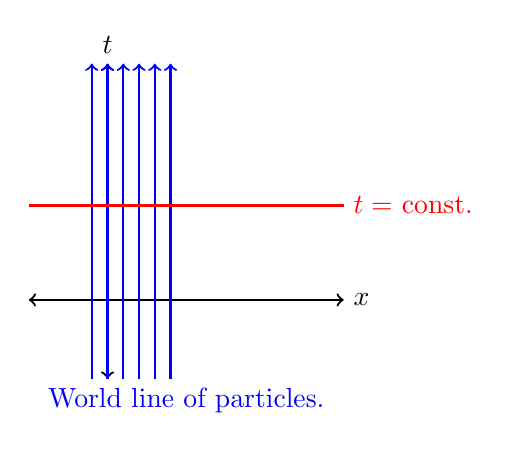
\begin{tikzpicture}
    % Draw axes
    \coordinate (nya) at (0, -1);
    \coordinate (pya) at (0, 3);
    \coordinate (nxa) at (-1, 0);
    \coordinate (pxa) at (3, 0);
    \draw [<->, thick] (nxa) -- (pxa);
    \draw [<->, thick] (nya) -- (pya);
    \node [above] (lpya) at (pya) {$t$};
    \node [right] (lpxa) at (pxa) {$x$};

    \draw [->, thick, blue] (-0.2, -1) -- (-0.2, 3);
    \draw [->, thick, blue] (0, -1) -- (0, 3);
    \draw [->, thick, blue] (0.2, -1) -- (0.2, 3);
    \draw [->, thick, blue] (0.4, -1) -- (0.4, 3);
    \draw [->, thick, blue] (0.6, -1) -- (0.6, 3);
    \draw [->, thick, blue] (0.8, -1) -- (0.8, 3);
    \draw [thick, red] (-1, 1.2) -- (3, 1.2);

    \node [blue, below] (l) at (1.0, -1) {World line of particles.};
    \node [red, right] (l) at (3, 1.2) {$t =$ const.};

\end{tikzpicture}
\end{center}

Thus this represents some sort of flux through a fixed time.

\[ \# \text{density} = \f{\# \text{particles}}{\De V} = \f{\# \text{particles}}{\De x \De A} \]

Whereas in the non co-moving frame the particles moving at speed $v_x$:


\begin{center}
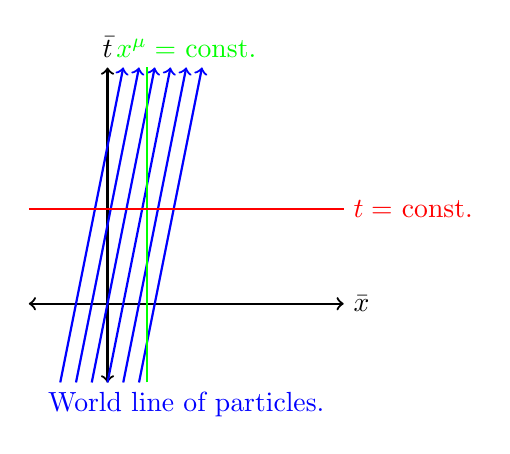
\begin{tikzpicture}
    % Draw axes
    \coordinate (nya) at (0, -1);
    \coordinate (pya) at (0, 3);
    \coordinate (nxa) at (-1, 0);
    \coordinate (pxa) at (3, 0);
    \draw [<->, thick] (nxa) -- (pxa);
    \draw [<->, thick] (nya) -- (pya);
    \node [above] (lpya) at (pya) {$\bar{t}$};
    \node [right] (lpxa) at (pxa) {$\bar{x}$};

    \draw [->, thick, blue] (-0.6, -1) -- (0.2, 3);
    \draw [->, thick, blue] (-0.4, -1) -- (0.4, 3);
    \draw [->, thick, blue] (-0.2, -1) -- (0.6, 3);
    \draw [->, thick, blue] (0, -1) -- (0.8, 3);
    \draw [->, thick, blue] (0.2, -1) -- (1.0, 3);
    \draw [->, thick, blue] (0.4, -1) -- (1.2, 3);
    \draw [-, thick, green] (0.5, -1) -- (0.5, 3);
    \draw [thick, red] (-1, 1.2) -- (3, 1.2);

    \node [blue, below] (l) at (1.0, -1) {World line of particles.};
    \node [red, right] (l) at (3, 1.2) {$t =$ const.};
    \node [green, above] (l) at (1.0, 3) {$x^\mu =$ const.};

\end{tikzpicture}
\end{center}

The relevant notion of relativistic number density is the notion of flux through the $x^\mu = $ const. We will introduce the ``\#-flux'' vector $N^\mu$. Where at rest,

\[ N^\mu = \mtrx{N \\ 0 \\ 0 \\ 0} \]

And under a boost such as in equation \eqref{eq:boost} where $v = v_x$,

\[ N^\mu = \mtrx{\ga N \\ \ga N v_x \\ 0 \\ 0} = N \mtrx{\ga \\ \ga v_x \\ 0 \\ 0} = N v^\mu \]

As a result, the magnitude of $N^\mu$ is given by,

\[ N^\mu N_\mu = N^2 v^\mu v_\mu = - N^2 \]

Now consider the mass density discussed above $\rho = M/V$. At rest we have $\rho = M/V$ with $E = M$ ($c=1$). Under a boost with $v_x$,

\[ \mtrx{E = m \\ 0 \\ 0 \\ 0} \ar \mtrx{\ga m = \bar{E} \\ m \ga v \\ 0 \\ 0} \]

Furthermore the volume under the boost becomes $V \ar \bar{V} = \f{1}{\ga} V$. So $\rho = M/V$ at rest becomes under a boost,

\[ \bar{\rho} = \ga^2 \rho \]

This is similar to the velocity terms but instead we have a $\ga^2$ term instead of $\ga$. Note that density is given by,

\[ \rho = \f{M}{V} = \f{n}{V} m \eq \label{eq:density}\]

Where $m$ is the mass of a single particle that should be considered the mass given by the four-momentum $p^\al$. The number density should be given by the four-number density $N^\be$. Using this interpretation, \eqref{eq:density} is expressed under the relativistic regime as,

\[ \rho \ar  N^\al \otimes p^\be = N v^\al \otimes m v^\be = m N v^\al \otimes v^\be = \rho v^\al \otimes v^\be \]

This new quantity $\rho v^\al \otimes v^\be$ will be called $T^{\al\be}$. At rest,

\[ v^\al = \mtrx{1 \\ 0 \\ 0 \\ 0} \]

Which gives $T^{00} = \rho$ and $T^{\al\be} = 0$ whenever $\al \neq 0$ or $\al \neq 0$. While in frame $(v_x)$,

\[ v^\al = \mtrx{\ga \\ v_x \\ 0 \\ 0} \]

Which gives,

\[ T^{00} = \ga^2 \rho \]

So why does this $\ga^2$ term keep showing up? Since $T^{00}$ is a tensor with two components the $\ga$ induced by the boost affects each of the components, namely $M$ and $V$. The boost affects the tensor for each index,

\[ T^{\al\be} \untext{\ar}{boost} {\Lam^\al}_\ga {\Lam^\be}_\de T^{\ga \de} = \bar{T^{\al\be}} \]

This tensor $T^{\al\be}$ is called the \textit{stress energy tensor} and will act as a source of gravity.

\begin{itemize}
    \item $T^{00}$: energy density
    \item $T^{0i}$: energy flux across $i$-th surface ($i = 1,2,3$)
    \item $T^{i0}$: momentum density ($i = 1,2,3$)
    \item $T^{ij}$: flux of $i$-th momentum through $j$-th surface ($i,j = 1,2,3$)
    \begin{itemize}
        \item this is known as the stress tensor that appears when particles have interactions with one another.
    \end{itemize}
\end{itemize}

\subsection{Properties of Stress Energy Tensor}

\textbf{symmetric:} $T^{\al\be} = T^{\be\al}$ \\

Here is a ``proof'' using dimensional arguments.
\begin{align*}
    T^{0i} &= \text{energy flux} \\
    &= \text{density of energy} \times \text{speed of flow} \\
    &= \text{density of mass} \times \text{speed of flow} \\
    &= \text{density of momentum}\\
    &= T^{i0}\\
\end{align*}

\textbf{conservation}: $\pder{}{x^\be} T^{\al\be} = 0$ \\

To demonstrate this conservation, think of conservation as ``what goes in and out of a box encodes the variations of what's inside the box.'' Consider a cube of side length $\ell$ aligned to a Cartesian coordinate system. Focusing on energy,

\[ \ell^3 \pder{}{t} T^{00} \note{variation of what's inside the box} \eq \label{eq:varin} \]

The rate of flow of energy of through each of the 6 faces of the cube is given by,

\[ \ell^2 T^{0x}(x=0) - \ell^2T^{0x}(x=\ell) + \ell^2 T^{0y}(y=0) - \ell^2T^{0y}(y=\ell) + \ell^2 T^{0z}(z=0) - \ell^2T^{0z}(z=\ell) \eq \label{eq:goesout} \]

Therefore by conservation \eqref{eq:varin} must equal \eqref{eq:goesout},

\[ \ell^3 \pder{}{t} T^{00} = \ell^2 \br{T^{0x}(x=0) - T^{0x}(x=\ell) +  T^{0y}(y=0) - T^{0y}(y=\ell) +  T^{0z}(z=0) - T^{0z}(z=\ell)} \]

Or more cleanly, dividing by $\ell^3$ and considering the limit as $\ell \ar 0$,

\[ \pder{}{t} T^{00} = \lim_{\ell \ar 0} \f{1}{\ell} \sum_{i=1}^{3} \br{T^{0i} (x^i = 0) - T^{0i} (x^i = \ell)} \]

Using the definition of partial derivatives,

\[ \pder{}{t} T^{00} = -\pder{}{x}T^{0x}-\pder{}{y}T^{0y}-\pder{}{z}T^{0z} \]

Or rearranged,

\[ \sum_{\al=1}^{3} \pder{}{x^\al}T^{0\al} = \pder{}{t} T^{0t} + \pder{}{x}T^{0x} + \pder{}{y}T^{0y} + \pder{}{z}T^{0z} = 0 \]

By Einstein summation convention,

\[ \pder{}{x^\al}T^{\be\al} = 0 \]

\subsection{Early Attempts at Relativistic Gravity}

Now what can we propose about gravity? Nordstrom in 1907 proposed to Einstein the idea of taking,

\[ \De \phi = 4 \pi G \rho \]

And replacing this with the D'Alembertian defined as \eqref{eq:alembert} and the stress energy tensor,

\[ \Box \phi = 4 \pi G {T^{\al}}_{\al} \]

This proposed theory is incorrect because this equation is linear. Here, gravity doesn't \textit{gravitate}.

In 1913, after hard work, Nordstrom proposed,

\[ \f{\Box \phi}{\phi} = 4 \pi G {T^{\al}}_{\al} \eq \label{eq:Nordstrom1913}\]

This theory is self consistent by it can be shown that under this theory, light doesn't bend with gravity. This has been proven to be true in our universe so it must also be wrong. \\

In 1914 however, Einstein and Fohker discovered that \eqref{eq:Nordstrom1913} could be recast as,

\[ R = {\ti{T}^{\al}}_\al \]

Where $R$ is the \textit{Ricci scalar curvature} from the study of Differential Geometry. This new theory is a geometrical theory. This is nice because it is a geometric, scalar, relativistic theory for gravity. Again this theory does not permit for the bending of light just as \eqref{eq:Nordstrom1913}; thus it must be wrong. Almost immediately afterwards, Einstein came out with his theory of general relativity in 1915.

\subsection{Equivalence Principles}

What is the difference between inertial mass and gravitational mass.

\begin{itemize}
    \item \textbf{Inertial mass}: Mass of an object measured by it's resistance to acceleration.
    \begin{itemize}
        \item An object with high inertial mass with accelerate less than objects with low inertial mass when subject to the same applied force
        \item $a = F / m_I$
    \end{itemize}
    \item \textbf{Gravitational mass}: Mass of an object that defines the gravitational force on a system.
    \begin{itemize}
        \item $m_G \vec{g} = \vec{F}_g$
    \end{itemize}
\end{itemize}

Note there are other forms of mass like relativistic mass and rest mass. \\

Experimentally inertial mass $m_I$ and gravitational mass $m_G$ have been found to be identical.

\subsubsection{Weak Equivalence Principle}

The weak equivalence principle states that test bodies fall with the same acceleration independently of their structure or composition. Formally,

\[ \f{m_I}{m_G} = 1 \]

This was experimentally verified by experiments in 1885 by Eötvös. Today we have verified this to $10^{-12}$, or $12$ decimal places. Exploring this idea,

\[ m_I \vec{a} = m_G \vec{g} \implies \vec{a} = \vec{g} \]

Uniform acceleration cannot be distinguished from a uniform gravitational field. \\

Consider the ISS orbiting at an altitude of $h = \SI{400}{\km}$. The gravitational field is roughly $90\%$ that of the surface gravitational field.

\[ g = \f{GM}{R+h} \]

Consider a particle in space characterized by position $\vec{x}$.

\[ m_I \dder{\vec{x}}{t} = m_G \vec{g} \]

Now consider a new frame $\vec{\chi}$ such that $\dder{\vec{\chi}}{t} = \vec{a}$ with coordinates in the old frame given by,

\[ \vec{x}' = \vec{x} = \vec{\chi} \]


\begin{center}
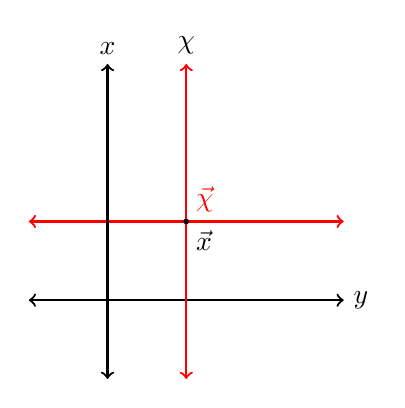
\begin{tikzpicture}
    % Draw axes
    \coordinate (nya) at (0, -1);
    \coordinate (pnya) at (1, -1);
    \coordinate (pya) at (0, 3);
    \coordinate (ppya) at (1, 3);
    \coordinate (nxa) at (-1, 0);
    \coordinate (pnxa) at (-1, 1);
    \coordinate (pxa) at (3, 0);
    \coordinate (ppxa) at (3, 1);
    \draw [<->, thick] (nxa) -- (pxa);
    \draw [<->, thick,red] (pnxa) -- (ppxa);
    \draw [<->, thick] (nya) -- (pya);
    \draw [<->, thick,red] (pnya) -- (ppya);
    \node [above] (lpya) at (pya) {$x$};
    \node [above] (lppya) at (ppya) {$\chi$};
    \node [right] (lpxa) at (pxa) {$y$};
    \node [right] (lppxa) at (ppxa) {$\ga$};
    \fill [red] (1,1) circle (1pt) node[above right] {$\vec{\chi}$};
    \fill [black] (1,1) circle (1pt) node[below right] {$\vec{x}$};

\end{tikzpicture}
\end{center}

Therefore,

\[ m_I \dder{\vec{x}'}{t} = m_I \dder{\vec{x}}{t} - m_I \dder{\vec{\chi}}{t} = m_G \vec{g} - m_I \vec{a} = m_G \br{\vec{g} - \vec{a}} \]

Which confirms again that uniform acceleration is indistinguishable from a uniform gravitational field. Also note that the first falling frame is an inertial frame.

\[ m_I \dder{\vec{x}'}{t} = m_G\br{\vec{g} - \vec{g}} = \vec{0} \]

\subsubsection{Tidal Forces}

Consider a spaceship large enough to experience the change in the gravitational field from one end to another. This force gradient causes stress and strain on the spaceship. These forces are called Tidal forces. To avoid tidal forces, only consider objects in a \textit{local inertial frame} where the field is \textit{uniform}.

\subsubsection{Einstein's Strong Equivalence Principle}

Free-falling in local inertial frame (where $\vec{g}$ is uniform), the results of all experiments will be indistinguishable from the results of the same experiments performed in a inertial frame in Minkowski spacetime.\\

Consider the case of a rocket with initially no acceleration $\vec{a} = \vec{0}$ and constant velocity $\vec{v} = \text{const}$. Another ship comes along and shoots a laser. Suppose there is a window on the left $w_L$ and a window on the right $w_R$. Now suppose the spaceship gets lucky and the laser passes through $w_L$ and then $w_R$ (a). From the perspective of the captain of the ship, the light moves as a straight line (b). Nothing too complicated. \\

\begin{center}
    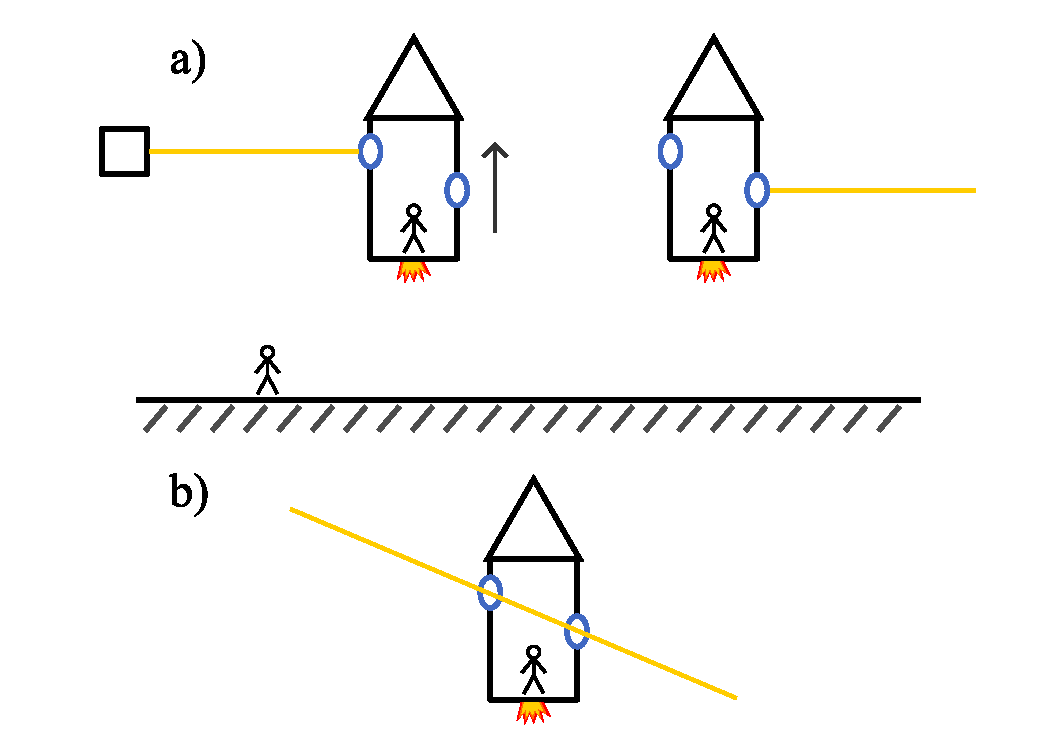
\includegraphics[scale=0.7]{figures/bend_light/constant_v.pdf}
\end{center}

Now consider the rocket moving with constant acceleration $\vec{a} =$ const (c). Additionally, the fired laser luckily misses the ship and passed through $w_L$ and then $w_R$. From the perspective of the captain, the light travels along a curved trajectory (d). Nothing too complicated. However by the Einstein's Strong Equivalence principle, this experiment must be identical to a stationary spaceship in a uniform gravitational field. Therefore, in a uniform gravitational field with everything else stationary, light \textbf{must} travel along a curved trajectory (e). Gravity bends light!

\begin{center}
    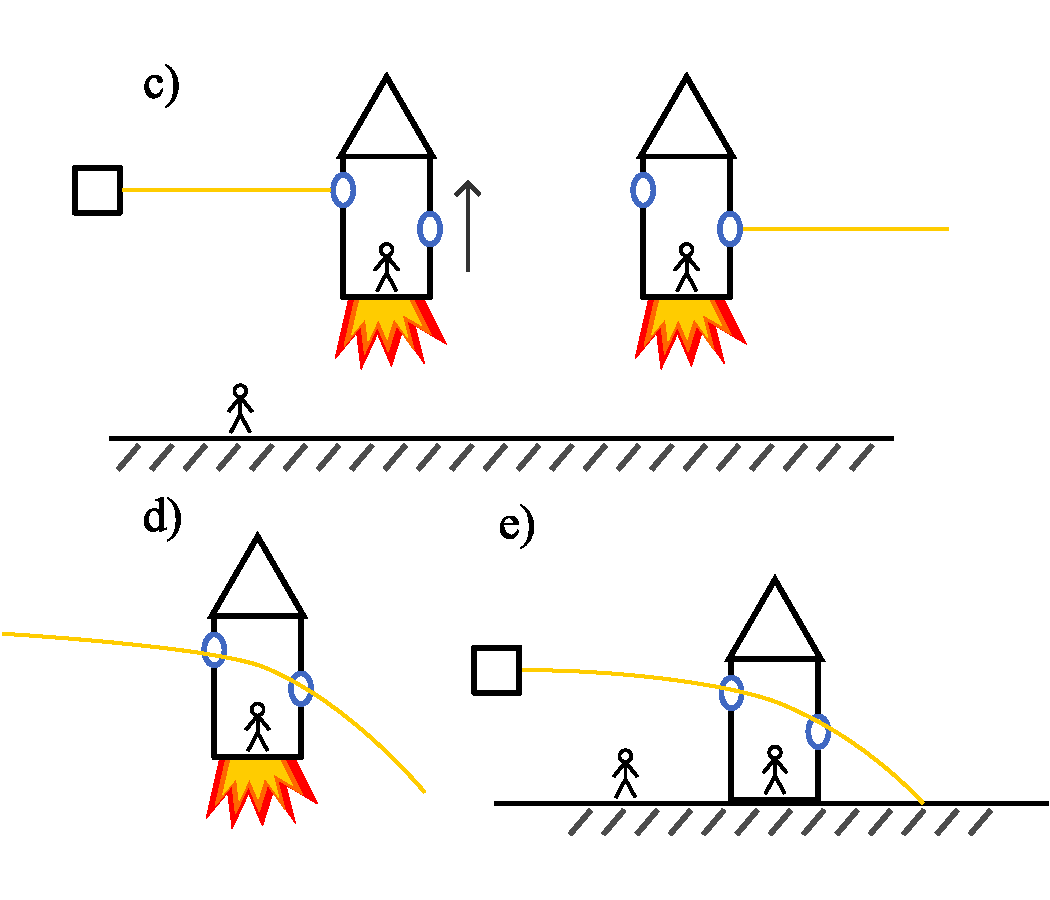
\includegraphics[scale=0.7]{figures/bend_light/constant_a.pdf}
\end{center}

We must be able to measure this effect. If the light falls in the gravitational field, it must gain energy $E = h \w$ and thus it will be blue shifted. Similarly, if the light climbs out of the gravitational field, it will lose energy and be red shifted. To explore this idea, consider a rocket with two individuals, one at the top of the rocket $(A)$ and one at the bottom $(B)$ (separated by height $h$). The rocket will be accelerating with $\vg$ in just the $\hz$ direction which gives,
\[ \ddot{z}_A = \ddot{z}_B = g \]

Therefore,
\[ z_A(t) = h + \f12 g t^2 \]
\[ z_B(t) = \f12 g t^2 \]

At $t=0$, $A$ sends a light signal to $B$ and is received by $B$ at time $t_1 > t_0 = 0$.
\[ ct_1 = z_A(0) - z_B(t_1) \]

At time $t = \De \tau_A$, $A$ emits another light signal to $B$ and it will be received at time $t_1 + \De \tau_B$,
\[ c\br{t_1 + \De \tau_B - \De \tau_A} = z_A\br{\De\tau_A} - z_B \br{t_1 + \De \tau_B} \]

With these two relations, we want to get an expression that relates $\De \tau_A$ to $\De \tau_B$. Considering a non-relativistic regime $c \gg 1$, and at 1st order in $\De \tau_i$ with $i = A,B$,
\[ \De \tau_B = \De \tau_A \br{1 - \f{gh}{c^2}} \]
This is strange. If there were no acceleration $\De \tau_B = \De \tau_A$. However, there is an extra factor of due to the acceleration $\vg$. Because of the acceleration, the second beam of light had to travel a farther distance making $\De \tau_B < \De \tau_A$. If $\De \tau$ is taken to be the period of light waves,
\[ \De \tau = \f{\la}{c} \]
Thus,
\[ \la_B = \la_A \br{1 - \f{gh}{c^2}} \]
Which gives use a similar relation between $\la_A$ and $\la_B$, namely $\la_B < \la_A$. This corresponds to a \textbf{blue shift}. Following a similar argument with $g \ar - g$ it becomes that $\la_B > \la_A$ which corresponds to a \textbf{red shift}. \\

However, by Einstein's Strong Equivalence Principle, the \textit{exact} same effect should occur while stationary under a uniform gravitational field $\vg$. We can perform this experiment on earth and measure the effect. This was known as the \textit{Pound Rebka experiment}. This effect is very small. On earth,
\[ \f{gh}{c^2} \sim \SI{e-15}{} \]

What does this experiment look like as a spacetime diagram,


\begin{center}
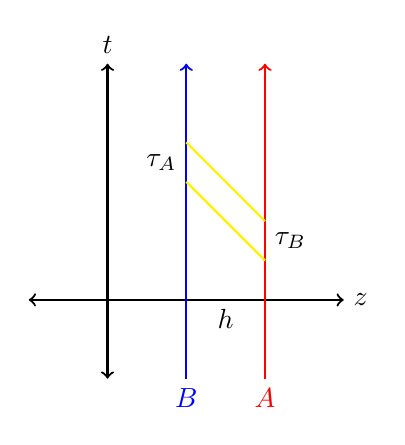
\begin{tikzpicture}
    % Draw axes
    \coordinate (nya) at (0, -1);
    \coordinate (pya) at (0, 3);
    \coordinate (nxa) at (-1, 0);
    \coordinate (pxa) at (3, 0);
    \draw [<->, thick] (nxa) -- (pxa);
    \draw [<->, thick] (nya) -- (pya);
    \node [above] (lpya) at (pya) {$t$};
    \node [right] (lpxa) at (pxa) {$z$};

    \draw [->, thick, blue] (1.0, -1) -- (1.0, 3);
    \draw [->, thick, red] (2.0, -1) -- (2.0, 3);
    \node [below, red] (la) at (2.0, -1) {$A$};
    \node [below, blue] (lb) at (1.0, -1) {$B$};

    \draw [thick, yellow] (2.0, 0.5) -- (1.0, 1.5);
    \draw [thick, yellow] (2.0, 1.0) -- (1.0, 2.0);
    \node [right] (lr) at (2.0, 0.75) {$\De \tau_B$};
    \node [left] (ll) at (1.0, 1.75) {$\De \tau_A$};
    \node [below] (lb) at (1.5, 0) {$h$};
\end{tikzpicture}
\end{center}

There is a problem here. Since the field $\vg$ is uniform, it must be that the two light rays are \textit{parallel}. Since the gravitational potential at $A$ and $B$ is given by $\phi_A, \phi_B$ and they are equal,
\[ \De \tau_B \approx \br{1 - \f{\phi_A - \phi_B}{c^2}} \De \tau_A = \De \tau_A \eq \label{eq:parallel} \]
However, we have just shown that,
\[ \De \tau_B < \De \tau_A \]
Which indicates that these lines are converging and thus should \textbf{not} be parallel. Nonetheless, this problem can be resolved when considering geometries like the surface of a sphere where \textit{great circles} are both parallel and intersecting. This convinced Einstein that he would have to learn \textit{differential geometry}. \\

Before moving to differential geometry, let us recall that for the Minkowski metric,
\[ \dif \tau^2 = \dif t^2 - \dif \vec{x}^2 \]

Now consider a modified metric,
\[ \dif \tau^2 = \br{1+2\phi(\vec{x})}\dif t^2 - \br{1-2\phi(\vec{x})}\dif \vec{x}^2 \eq \label{eq:modmetric}\]

This is known as the \textit{static weak field metric} where $\phi$ is the gravitational potential. Can this metric recover some of the issues discussed above? If $A$ and $B$ are at rest $\De \vec{x}^2 = 0$,
\[ \De \tau_A^2 = \br{1+2\phi(x_A)}\De t^2 \]
\[ \De \tau_B^2 = \br{1+2\phi(x_B)}\De t^2 \]
Which gives,
\[ \De \tau_A^2 = \f{1+2\phi(x_A)}{1+2\phi(x_B)}\De \tau_B^2 \]
Where a Taylor series expansion gives,
\[ \De \tau_A \approx \br{1+\phi(x_A)-\phi(x_B)}\De \tau_B \]
Which can be seen to mimic \eqref{eq:parallel}. This motivates how gravity can be described as a modified metric which in turn implies a gravity affects the space in which the system lives.

\section{Differential Geometry}

We known the flat $\R^n$ space very well. How can be relate different geometries back to $\R^n$. Consider the surface of the earth. How can we measure \textit{where we are}? Consider someone living in Waterloo, they might have a map that has coordinates describing where they are. Similarly for someone in Toronto with a different map, they would have coordinates that describe where they are. In order for these two people to communicate, there needs to be a translation between the coordinates on one map to another. This is the spirit of differential geometry. By stitching together maps (charts), we can get a description of geometry through the non-trivial overlaps between adjacent maps. At any given space in our manifold, we can define a set of tangent vectors which span a \textit{tangent bundle} or tangent plane. These tangent planes can form a vector space throughout the geometry. Through these spaces, we can define co-vectors and thus tensors like metrics without these spaces. We will also explore the idea of a derivative of a tensor that relates difference tangent planes.

\subsection{Definitions}

\textbf{Open Ball in $\R^n$}: An open ball in $\R^n$ centered at $y$ is the set of all $x \in \R^n$ such that,
\[ \bc{x \in \R^3 \mid \text{for a given } y \in \R^n, \abs{x - y} < R \text{ with } \abs{x-y}^2 = \sum_i \br{x-y}_i^2} \]
Where $R \in \R_{>0}$.\\

\textbf{Open set}: An open set in $\R^n$ is built from the union of open balls.

\textbf{Chart}: Let $M$ be a set not necessarily $\R^n$. A \textbf{chart} or coordinate system $\br{\phi, \mathcal{U}}$ consists of a subset $\mathcal{U}$ of $M$ with a one-to-one map,
\[ \phi : \mathcal{U} \ar \R^n \]
Such that $\phi\br{\mathcal{U}} = V$ is an open set (in $\R^n$). We can say that $\mathcal{U} = \phi^{-1}\br{V}$. We can use $V$ to induce the topology of our topological space. By notation, we usually note $\phi(p)$ where $p \in \mathcal{U}$, as,
\[ \phi\br{p} \defined x^{\mu} \br{p} \note{$\phi$ acts as the \textit{notion} or coordinates in $\R^n$ at $p$} \]

\textbf{Atlas}: An atlas is a collection of charts $\br{\mathcal{U}_\al, \phi_\al}$ such that the union of all $\mathcal{U}_\al$ covers all of $M$,
\[ \cup_\al \mathcal{U}_\al = M \]
If two charts happen to overlap, (i.e. $\mathcal{U}_\al \cap \mathcal{U}_\be \neq \emptyset$), then the map $\phi_\al \circ \phi_\be^{-1}$ takes points in $\phi_\be \br{\mathcal{U}_\al\cap\mathcal{U}_\be}$ to $\phi_\al \br{\mathcal{U}_\al\cap\mathcal{U}_\be}$. We say that the chart is $C^\inf$ (or smooth) if $\phi_\al$ is $C^\inf$ (infinitely differentiable). If all the charts are $C^\inf$ then $\phi_\al \circ \phi_\be^{-1}$ and its inverse are $C^\inf$. \\

\textbf{Manifold}: A manifold is a set $M$ equipped with a maximal atlas (i.e. the one that contains all the possible charts). If the atlas is defined by $\phi_\al : M \ar \R^n, \forall \al$ then $M$ is a manifold of dimension $n$.

\subsubsection{Examples of Manifolds}

Consider $S_1$ the circle in the plane $\R^2$,

\[ S^1 = \bc{\br{x,y}\in \R^2 \mid x^2 + y^2 = 1} \]

Now consider the open sets consisting of $y>0$ (red) and $y<0$ (green), as well as $x>0$ (yellow) and $x<0$ (blue).

\begin{center}
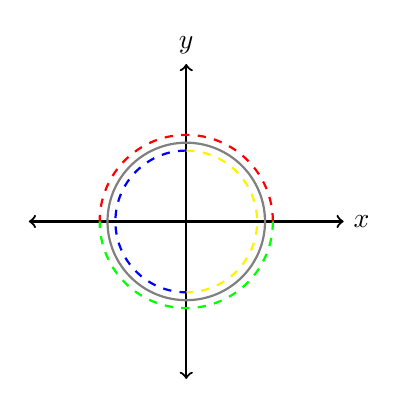
\begin{tikzpicture}
    % Draw axes
    \coordinate (nya) at (0, -2);
    \coordinate (pya) at (0, 2);
    \coordinate (nxa) at (-2, 0);
    \coordinate (pxa) at (2, 0);
    \draw [<->, thick] (nxa) -- (pxa);
    \draw [<->, thick] (nya) -- (pya);
    \node [above] (lpya) at (pya) {$y$};
    \node [right] (lpxa) at (pxa) {$x$};

    \draw [thick, gray] (0,0) circle (1);
    \draw [thick, red,dashed] (1.1,0) arc (0:180:1.1);
    \draw [thick, green,dashed] (1.1,0) arc (0:-180:1.1);
    \draw [thick, yellow,dashed] (0,0.9) arc (90:-90:0.9);
    \draw [thick, blue,dashed] (0,0.9) arc (90:270:0.9);
\end{tikzpicture}
\end{center}

The four points of the form, $(x,y) = (1,0),(-1,0),(0,1),(0,-1)$, all belong to a single open set on $S^1$. However, for regions that belong to two separate open sets, we need a map that takes us from one open set to the next. For example, to map from yellow to red,
\[ y\tsb{red} = \sqrt{1 - x\tsb{yellow}^2} \eq \label{eq:circle}\]
This acts as the form $\phi_x \circ \phi_y^{-1} \br{x}$. Is this composite map $C^{\inf}$? Note that \eqref{eq:circle} is only not differentiable at $x = 0$. However, this point doesn't not belong the intersection of the red and yellow regions. Therefore, \eqref{eq:circle} is $C^\inf$. More more, see Caroll's book (online) for differential geometry.

\subsection{Tangent Vectors}

Before we defined the notion of tangent vectors, we will need to first discuss trajectories.

\subsubsection{Trajectories}

\newcommand{\CC}{\mathcal{C}}

\textbf{Definition}: A $C^\inf$ curve in a manifold $M$ is a map $\mathcal{C} : \R \supset I \ar M, \tau \ar \mathcal{C}\br{\tau}$ were $I$ is an interval on $\R$ such that,
\[ \forall \al : \phi_\al \circ \mathcal{C} \text{ is a $C^\inf$ map} \]
For points $p$ in $M$ get mapped to $x^\mu(P)$ in $\R^m$ through $\phi_m$ along the interval $I$ parametrized by $\tau$. In summary, we take an interval $I$ in $\R$ and then map it to a trajectory in $M$ using $\mathcal{C}$ which is taken locally to $\R^n$ by $\phi_\al$.
\[ \mathcal{C} : I \ar M \]
\[ \phi_\al \circ \mathcal{C}(\tau) \defined x^\mu(\tau) \]
\textbf{Definition}: We note $\mathcal{C}^\inf\br{M}$ the \textbf{algebra} of $C^\inf$ functions of the form $f : M \ar \R$, with point-wise product given by,
\[ \br{f_1 \cdot f_2}\br{p} = f_1\br{p}f_2\br{p} \]
Where $P \in M$.\\
\textbf{Definition}: Let $\mathcal{C}: I \ar M$ be a smooth curve with $\mathcal{C}(0) = p$. The \textbf{tangent vector} to $\mathcal{C}$ at $p$ is the linear map $X_p:\mathcal{C}^\inf\br{M} \ar R$ given by,
\[ X_p\br{f} = \der{}{\tau}f\br{\mathcal{C}\br{\tau}}|_{\tau=0} \]
Notation:
\[ f \circ \CC = f \circ \phi_\al^{-1} \circ \phi_\al \circ \CC \]
Using the combination $F = f \circ \phi^{-1}_\al$ which is a map $F: \R^n \ar \R$ (since $\phi_\al \circ \CC: I \ar R^n$) which gives a more convenient expression,
\[ f \circ \CC\br{\tau} = F\br{x^\mu\br{\tau}} \]
Using the coordinate system, this becomes,
\begin{align*}
X_P\br{f} &= \der{}{\tau}\bre{F \br{x^\mu\br{\tau}}}_{\tau=0} \\
&= \untext{\bre{\der{x^\mu}{\tau}}_{\tau = 0}}{components} \untext{\bre{\pder{}{x^\mu} F \br{x^\mu}}_{p}}{basis} \note{Chain rule.} \\
\end{align*}
Exploring this notation motivates the separation of the coordinates and basis of the tangent vector $X_p \br{f}$. Focusing on the specific curves $\CC_k\br{\tau}$ such that,
\[ x^\mu \br{\CC_k\br{\tau}} = \br{x^0\br{p}, \ldots, x^k\br{p} +\tau, \ldots, x^n\br{n}}\]
This addition of $\tau$ along each direction allows for the ``exploration'' of the $k$-th direction by an amount $\tau$.
\[ \CC_1 : \br{x(p) + \tau, y\br{p}} \]
\[ \CC_2 : \br{x(p) , y\br{p}+ \tau} \]
This gives the form,
\[  \der{x^\mu}{\tau}\br{\CC_k\br{\tau}}|_{\tau=0} = {\de^\mu}_k \]
So that the tangent vector of $\CC_k$ is $\pder{}{x^k}|_p$. \\
\textbf{Definition}: The set of all tangent vectors at a point $p$ is the tangent plane $T_pM$ at $p$. \\

\textbf{Theorem}: If $M$ has dimension $n$ then $T_pM$ has dimension $n$, making $T_pM \sim \R^n$. The basis of $T_pM$ is given by $\pder{}{x^\mu} |_p$.\\

\textbf{Comments}:
\begin{itemize}
    \item In the tangent space $T_pM$, a general vector is $X = X^\mu \pder{}{x^\mu} = X^\mu \di_\mu$ (noting, down in the $\di$ term means up in the denominator by notation).
    \item The basis $\pder{}{x^\mu}$ is coordinate dependent. Another coordinate system could be $\pder{}{y^\mu}|_p$.
\end{itemize}

These different basis are of course related by the Jacobian (Wald p.17),
\[ \pder{}{x^\mu}\bigg\rvert_p = \pder{y^\al}{x^\mu}\bigg\rvert_p \pder{}{y^\al}\bigg\rvert_p \]

So a generic vector in $T_pM$ is $X = X^\mu \pder{}{x^\mu} = \ti{X}^\mu \pder{}{y^\mu}$. How do the components $X^\mu$ relate to $\ti{X}^\mu$?

\[ X^\mu \pder{}{x^\mu} = \ti{X}^\al \pder{}{y^\al} = X^\mu \pder{y^\al}{x^\mu} \pder{}{y^\al} \]
This gives the relation,
\[ X^\mu \ar \ti{X}^\mu = X^\al \pder{y^\mu}{x^\al}\]

\textbf{Definition}: We define a cotangent space $T^*_pM$ as the set of linear maps $T_pM \ar \R$. It has dimension $n$. We note the basis of $T^*_pM$ by $\dif x^\mu$ (sometimes called a form).
\[ \dif x^\mu \br{\di_\al} = {\de^\mu}_\al \note{analogously to $f^\mu\br{e_{\al}} = {\de^\mu}_\al$} \]

\textbf{Remark}: Both the tangent space $T_pM$ and cotangent space $T^*_pM$ are in general not contained in the manifold $M$. Only in flat Minkowski space is this is case.

\subsection{Tensor Calculus}

\textbf{Definition}: A tensor of type $\br{r,q}$ on $T_pM$ is a multi-linear map:
\[ T: \underbrace{T^*_pM \times \cdots \times T^*_pM}_{r} \times \underbrace{T_pM \times \cdots \times T_pM}_{q} \ar \R \]

\textbf{Examples}:
\begin{center}
\begin{tabular}{|c|c|}
    \hline
    Tensor & Rank \\
    \hline
    $X^\mu$ & $\br{1,0}$ \\
    $X_\mu$ & $\br{0,1}$ \\
    $g_{\al\be}$ & $\br{0,2}$ \\
    \hline
\end{tabular}
\end{center}

\textbf{Definition}: A type $\br{0,2}$ tensor $g_{\al\be}$ which is non-degenerate ($v^\mu g_{\mu\al} w^\al = 0 \quad \forall w^\al \implies v^\mu = 0$) and symmetric ($g_{\al\be} = g_{\be\al}$) is a metric tensor. The notion of signature defined in $\R^n$ is the same as before.

\textbf{Definition}: We consider the union of the tangent spaces $T_pM$ for all $p\in M$ (respectively $T^*_pM$). We note,
\[ T\br{M} = \bigcup_{p\in M} T_p M \qquad T^*\br{M} = \bigcup_{p\in M} T^*_p M \]
A \textbf{vector field} is a map $X : M \ar T(M), p \ar X_p$. Likewise a \textbf{tensor field} is,
\[ T : M \ar T^*(M) \times \cdots \times T^*(M) \times T(M) \cdots \times T(M) \]
Or for a specific point $p$, $p \ar T_p$. From now on we will work with tensor fields. We extend all the formalism done in the Minkowski space.
\begin{itemize}
    \item Metric gives us the norm of vectors $ v^\al g_{\al\be} v^\be = L $ where $v^\al,g_{\al\be}$ are associated with a tangent plane at a point $T_pM$
    \item The sign of $L$ determines the type of vector
    \begin{itemize}
        \item $L > 0 \ar V^\al$ is space-like
        \item $L = 0 \ar V^\al$ is light-like
        \item $L < 0 \ar V^\al$ is time-like
    \end{itemize}
    \item A curve in $M$ has type that follows from the tangent vector $v^\al$
    \begin{itemize}
        \item $M$ is space-like if tangent vector is space-like
        \item $M$ is light-like if tangent vector is light-like
        \item $M$ is time-like if tangent vector is time-like
    \end{itemize}
    \item The arclength of a curve is given by,
\end{itemize}

\[ \tau = \int \sqrt{\abs{\der{x^\mu}{\ell}g_{\mu\al}\der{x^\al}{\ell}}} \]
Where $\ell$ is a curvilinear parameter of the curve and $\der{x^\mu}{\ell}$ is the tangent vector. The line element is given by,
\[ \dif \tau^2 = \abs{g_{\al\mu}\dif x^\mu \dif x^\al} \]

We will physically interpret the arclength $\tau$ to be proper time.
\begin{itemize}
    \item $\der{x^\mu}{\tau} = $ tangent vector $=$ relativistic velocity
    \item $\dder{x^\mu}{\tau} = $ relativistic acceleration
\end{itemize}

How can we generalize Newton's law $\vF_g = m_I \va$. Using the scalar gravitational field,
\[ - m_G \vdel \phi = m_I \va \]

Since the weak equivalence principle gives us $m_G = m_I$. Therefore,
\[ - \vdel \phi = \va \]
What is the relativistic version? Like us assume we are in a \textit{free falling} frame given by coordinate $\xi^\al$. Then according to Einstein's strong equivalence principle, the acceleration is just zero,
\[ a^\mu = \dder{\xi^\mu}{\tau} = 0 \]
Since we are in a free falling frame, physics must behave like the physics in Minkowski spacetime. The line element is given by,
\[ \dif \tau ^2 = \eta_{\mu\al} \dif \xi^\mu \dif \xi^\al \]
Where $\eta_{\mu\al}$ is the Minkowski metric. Now let us perform a change of coordinates and move \textit{away} from the free falling frame.
\[ \xi^\mu \ar x^\mu \]
This transformation is transformed by the Jacobian. However notice that,
\[ \dder{\xi^\mu}{\tau} = \der{v^\mu}{\tau} \]
But as shown on the assignment, $v^\mu$'s coordinates do not transform well. There are extra terms generated.
\[ \pder{\xi^\mu}{x^\al} \note{Jacobian} \]
\[ \pder{x^\al}{\xi^\mu} \note{Inverse Jacobian} \]
Which gives via the inverse relation,
\[ \pder{\xi^\mu}{x^\al}\pder{x^\al}{\xi^\rho} = {\de^\mu}_\rho \]
Which gives,
\begin{align*}
    \dif \tau^2 &= \eta_{\mu\al} \dif \xi^\mu \dif \xi^\al \\
    &= \eta_{\mu\al} \pder{\xi^\mu}{x^\ga}\pder{\xi^\mu}{x^\be}\dif x^\ga \dif x^\be \\
    &= g_{\ga\be}\dif x^\ga \dif x^\be
\end{align*}
But if we have the velocity to be,
\[ v^\mu = \der{\xi^\mu}{\tau} = \pder{\xi^\mu}{x^\al} \der{x^\al}{\tau} \]
This implies acceleration is given by \textit{product rule},
\begin{align*}
0 &= a^\mu  \\
&= \der{}{\tau} v^\mu \\
&= \der{}{\tau} \br{\pder{\xi^\mu}{x^\al} \der{x^\al}{\tau}} \\
&= \der{x^\al}{\tau}\der{}{\tau} \br{\pder{\xi^\mu}{x^\al} } + \pder{\xi^\mu}{x^\al}\der{}{\tau} \br{ \der{x^\al}{\tau}} \note{Product rule.}\\
&= \der{x^\al}{\tau} \f{\di^2\xi^\mu}{\di x^\al\di x^\be}\der{x^\be}{\tau} + \pder{\xi^\mu}{x^\al}\dder{x^\al}{\tau} \note{Chain rule.}\\
\end{align*}
Multiply by the inverse Jacobian on both sides (and send $\al \ar \ga$ for ease of notation),
\[ 0 = \dder{x^\al}{\tau}  + \underbrace{\pder{x^\al}{\xi^\mu} \f{\di^2\xi^\mu}{\di x^\ga\di x^\be}}_{{\Ga^\al}_{\ga\be}}\der{x^\ga}{\tau}\der{x^\be}{\tau} \]
Where ${\Ga^\al}_{\ga\be}$ are called the Christoffel symbols. Notice that they are symmetric in the lower indices,
\[ {\Ga^\al}_{\ga\be} = {\Ga^\al}_{\be\ga} \]
There is relationship between ${\Ga^\al}_{\be\ga}$ and the metric which and the metric transformation,
\[ g_{\al\be} = \eta_{\mu\nu} \pder{\xi^\mu}{x^\al}\pder{\xi^\nu}{x^\be} \]
Which can be derived to be,
\[ {\Ga^\al}_{\ga\be} = \f12 g^{\nu\sigma}\br{\pder{g_{\mu\nu}}{x^\lambda} + \pder{g_{\lambda\nu}}{x^\mu} - \pder{g_{\mu\lambda}}{x^\nu}} \]
This implies,
\[ \dder{x^\al}{\tau} + {\Ga^\al}_{\ga\be} \der{x^\ga}{\tau} \der{x^\be}{\tau} \]
Which implies the relationship between acceleration and the change of coordinates characterized by ${\Ga^\al}_{\ga\be}$,
\[ a^\al = - {\Ga^\al}_{\ga\be}  v^\ga  v^\be\]

Can we retrieve in a non relativistic limit $\va = - \vdel \phi$? To do this we need to convert show the analogy of this geometrical equation,
\[ \ti{a}^\mu = \dder{x^\mu}{\tau} + {\Ga^{\mu}}_{\al\be} v^\al v^\be = 0 \eq \label{eq:accelgrav} \]
To the gravitational force equation,
\[ \va = - \vdel \phi \eq \label{eq:gravforce}\]
In order to reveal this connection, we will perform a non-relativistic limit to \eqref{eq:accelgrav} and a weak field stationary metric to \eqref{eq:gravforce}. Using $c=1$ and $\abs{\vv} \ll 1$ we have,
\[ v^\al = \mtrx{\ga \\ \ga v^1 \\ \ga v^2 \\ \ga v^3} \]
Making for $i = 1,2,3$, the real space velocity components $v^i/v^0$. Therefore we have $\abs{\vv/v_0} \ll 1$. The non-relativistic limit becomes,
\[ \abs{\vv} \ll v_0 \]
So therefore the time components dominate,
\[ {\Ga^\al}_{\al\be}v^\al v^\be \approx {\Ga^\al}_{00}v^0 v^0 \]
By definition of ${\Ga^\al}_{\al\be}$,
\[ {\Ga^\al}_{00} = -\f12 g^{\mu\al} \pder{g_{00}}{x^\al}  \eq \label{eq:timedominant}\]
Now we will perform a weak field stationary metric on \eqref{eq:gravforce}. Therefore for a general metric $g_{\al\be}$ we can treat it as a Minkowski metric plus a tiny perturbation $\abs{h_{\al\be}} \ll 1$,
\[ g_{\al\be} = \eta_{\al\be} + h_{\al\be} \eq \label{eq:weakfield} \]
As such we will work in a 1st order approximation in $h_{\al\be}$. What is $g^{\al\be}$?
\[ g^{\al\be}g_{\be\ga} = {\de^{\al}}_\ga \]
Subbing in \eqref{eq:weakfield} the LHS becomes,
\[ \br{\eta^{\al\be} - h^{\al\be}}\br{\eta_{\be\ga} + h_{\be\ga}} = \eta^{\al\be}\eta_{\be\ga} - h^{\al\be}\eta_{\be\ga} + \eta^{\al\be}h_{\be\ga} - h^{\al\be}h_{\be\ga} \]
Noting that $\eta^{\al\be} - h^{\al\be}$ is a candidate for the inverse metric which will be justified after the fact for a first order approximation. $h^{\al\be}h_{\be\ga}$ is second order in $h_{\al\be}$ so it is negligible. Also, $\eta^{\al\be}\eta_{\be\ga} = {\de^\al}_\ga$ by inverse property and the remaining terms cancel out since $h_{\al\be}$ must be symmetric (because it's a metric). Therefore out inverse candidate is given by the assumed,
\[ g^{\al\be} = \eta^{\al\be} - h^{\al\be} \]
Then using \eqref{eq:timedominant}
\begin{align*}
{\Ga^\mu}_{00} &= -\f12 g^{\mu\al} \pder{g_{00}}{x^\al}\\
&= -\f12 \br{\eta^{\mu\al} - h^{\mu\al}} \pder{}{x^\al}\br{\eta^{00} + h^{00}}\\
&= -\f12 \br{\eta^{\mu\al} - h^{\mu\al}} \pder{}{x^\al}\br{h^{00}} \note{Since $\eta^{00} = -1$ in Cartesian coords}\\
&= -\f12 \br{\eta^{\mu\al}} \pder{}{x^\al}\br{h^{00}} \note{Ignoring terms that are second order in $h_{\al\be}$}\\
\end{align*}
Recall when discussing the bending of light, \eqref{eq:modmetric} reproduced the right results. We should expect the following metric,
\[ g_{\al\be} = \eta_{\al\be} - 2 \de_{\al\be}\phi\br{\vx} \]
to hold. This motivates $h_{\al\be}$ to take the form $2 \de_{\al\be}\phi\br{\vx}$. Note that this metric is \textit{stationary}. Meaning that,
\[ \di_t h_{\al\be} = \di_t 2 \de_{\al\be}\phi\br{\vx} = 0 \]
Therefore,
\[ \ti{a}^\mu = \dder{x^\mu}{\tau} = - {\ga^{\mu}}_{\al\be} v^\al v^\be \approx - {\ga^{\mu}}_{00} v^0 v^0 \]
Becomes,
\[ \ti{a}^\mu = + \f12 \eta^{\mu\al}\br{\pder{}{x^\al}h_{00}}v^0v^0 \]
Which has time component $\mu = 0$,
\[ \ti{a}^0 = + \f12 \eta^{0\al}\br{\pder{}{x^\al}h_{00}}v^0v^0 = 0\]
Since $h_{\al\be}$ is stationary. It also has space components $i = 1,2,3$,
\[ \ti{a}^i = \dder{x^i}{\tau} = + \f12 \eta^{i\al}\br{\pder{}{x^\al}h_{00}}v^0v^0\]
Noting that the $v^0$ terms are (again with $c=1$),
\[ v^0 = \der{x^0}{\tau} = \der{t}{\tau} \]
Therefore,
\[ \dder{x^i}{\tau} = + \f12 \eta^{i\al}\br{\pder{}{x^\al}h_{00}}\br{\der{t}{\tau}}^2 \]
In the non-relativistic limit $\tau \ar t$. Therefore,
\[ \dder{x^i}{t} = + \f12 \eta^{i\al}\br{\pder{}{x^\al}h_{00}} \]
Noting by motivation above that $h_{00} = - 2\phi\br{\vx}$,
\[ \dder{x^i}{t} = + \f12 \eta^{i\al}\br{\pder{}{x^\al}\br{- 2\phi\br{\vx}}} \]
\[ \dder{x^i}{t} = - \eta^{i\al}\br{\di^i\phi} \]
Which by sifting of $\al = i, \eta^{ii} = 1$,
\[ \dder{x^i}{t} = - \di^i\phi \]
\[ \vec{\ti{a}} = - \vdel\phi \]
Therefore Gravity is not a force by a curvature or geometry of spacetime.
\subsection{Differential Geometry Summary}
In summary, our aim is to take an interval $I \subset \R$ parametrized by curvilinear parameter $\tau$ and embed it into the manifold $M$. In doing so, we ascribe for every $\tau$ a point $\mathcal{C}\br{\tau}$ in the manifold. This creates a curve in $M$.Since dealing directly with abstract points $p$ in the manifold is difficult, we will use charts to assign coordinates to the points $\mathcal{C}\br{\tau}$ by using $\phi$ which gives $x^\mu \br{\mathcal{C}\br{\tau}}$. Now to discuss smoothness of this curve, we need to use $F : f \circ \phi^{-1} : \R^m \ar \R$. Moreover, we can define an $X : \mathcal{C}^\inf \br{M} \ar \R$ to map from $f$ (which makes points in $M$ to $\R$ regardless of the dimension of $M$) to real numbers $\R$. Then,
\[ X \br{f} = \der{x^\mu}{\tau}\bigg\rvert_{\tau = 0} \pder{F}{x^\mu}\bigg\rvert_{\phi\br{p}} \]
This motivates the convenient tensor notation for $X$,
\[ X = X^\mu \di_\mu \]
\subsection{Covariant Derivative}
Let us continue to explore,
\[ m \va = \vF_g \]
And manipulate the derived expression,
\[ m \br{a^\mu + {\Ga^\mu}_{\al\be}v^\al v^\be} = 0 \]
Using the definition of $a^\mu$,
\[ \dder{x^\mu}{\tau} = \der{x^\al}{\tau} \pder{}{x^\al} \der{x^\mu}{\tau} = v^\al \pder{}{x^\al} v^\mu \]
Therefore,
\[ v^\al \pder{}{x^\al} v^\mu + {\Ga^\mu}_{\al\be}v^\al v^\be = 0\]
Which suggests,
\[ v^\al \br{\pder{}{x^\al} v^\mu + {\Ga^\mu}_{\al\be} v^\be} = 0 \]
Where the \textbf{covariant derivative} is given by, $\del_\al v^\mu$ where,
\[ \del_\al v^\mu = \pder{}{x^\al} v^\mu + {\Ga^\mu}_{\al\be} v^\be \]
This leads to something known as the \textbf{geodesic equation},
\[ v^\al \del_\al v^\mu = 0 \]
With $v^\mu$ being the tangent vector to the geodesic. More formally, the covariant derivate is the \textit{notion of derivative that transforms well under a change of coordinates}.\\

\textbf{Definition}: The \textit{covariant derivate} $\del$ on a manifold $M$ is a map $\del : T\br{M} \times T\br{M} \ar T\br{M}$ where $T\br{M} = \cup_{p \in M}T_pM$. It takes two vector fields $X, Y$ and maps it to $\del_X Y$. It does so such that the following properties hold,
\[ \del_{fX + gZ}Y =  f\del_{X}Y + g\del_{Z}Y  \note{Linearity} \eq \label{eq:linearitycov1} \]
\[ \del_{X}\br{Y + Z} =  \del_{X}Y + \del_{X}Z  \note{Linearity} \eq \label{eq:linearitycov2}\]
\[ \del_{X}\br{fY} =  \br{\del_{X}f}Y + f\br{\del_{X}Y}  \note{Product rule}\]
Where $X,Y : \mathcal{C}^\inf\br{M} \ar \R$,
\[f\ar X\br{f} = X^\mu \di_\mu f \]
Where $f$ comes from $F = f \circ \phi^{-1}$. The covariant derivative on a scalar $\del_{X}f$ is given by,
\[ \del_{X}f \defined X\br{f} = X^\mu \pder{}{x^\mu}f \]
Consider a generic $\del_{X}Y$ and take $X$ in the basis $X^\mu = \de^{\al\mu}$ so that,
\[ X = X^\mu \di_\mu = \de^{\al\mu} \di_\mu = \di_\al \]
Which suggests the notation for this particular basis,
\[ \del_\al Y \defined \del_{e_\al} Y \]
What is $\del_X Y$ in terms of the basis $e_\al$ of $T_p\br{M}$? Let us examine the action of the covariant derivative directly on the basis. Since this quantity $\del_\al e_\be$ is an element in the tangent space, it should be able to be written with respect to the basis $e_\al$,
\[ \del_\al e_\be \defined {\Ga^\ga}_{\al\be}e_\ga \]
Where ${\Ga^\ga}_{\al\be}$ is the coefficients of the \textit{connection} in the basis $e_\al$. The \textit{Christoffel symbols} are an example. Therefore what is the expression for $\del_X Y$? Writing $X, Y$ as their basis expansions (noting that $Y = Y^\al e_\al$ where $Y^\al$ are each functions because $Y$ is a vector field and $e_\al$ are just basis vectors),
\[ \del_X Y = \del_{X^\al e_\al}\br{Y^\be e_\be} \]
Where $X^\al, Y^\be$ are components of the vector field at a point in the manifold with respect to the corresponding basis $e_\al \in T_p\br{M}$. They are functions of $p$ the point in the manifold. Using \eqref{eq:linearitycov1},
\[ \del_X Y = X^\al\del_{e_\al}\br{Y} \eq \label{eq:expandx} \]
Now using \eqref{eq:linearitycov2} to expand out $Y$ into it's components,
\begin{align*}
\del_X Y &= \del_{X}\br{Y^\be e_\be} \\
&= \del_X \br{Y^0 e_0 + Y^1 e_1 + \cdots } \\
&= \del_X \br{Y^0 e_0} + \del_X \br{Y^1 e_1} + \cdots \\
&= X\br{Y^0} e_0 + Y^0 \del_X e_0 + X\br{Y^1}e_1 + Y^1 \del_X e_1 + \cdots \\
&= X\br{Y^\be} e_\be + Y^\be \del_X e_\be \eq \label{eq:expandy}
\end{align*}
Where $X\br{Y^\be}$ is given by,
\[ X\br{Y^\be} = X^\al e_\al \br{Y^\be} \]
Which more specifically can be written using the basis for the tangent space $e_\al = \pder{}{x^\al}$,
\[ X\br{Y^\be} = X^\al \pder{}{x^\al} \br{Y^\be} \]
Furthermore using \eqref{eq:expandx} we can expand out the second term in \eqref{eq:expandy}.
\begin{align*}
\del_X Y &= X\br{Y^\be} e_\be + Y^\be \del_{X^\al e_\al} e_\be \note{Expand $X$}\\
&= X\br{Y^\be} e_\be + Y^\be X^\al \del_{e_\al} e_\be \\
&= X\br{Y^\be} e_\be + Y^\be X^\al \del_{\al} e_\be \note{By notation}\\
&= X\br{Y^\be} e_\be + Y^\be X^\al {\Ga^\mu}_{\al\be} e_\mu \note{Using the connection $\Ga$} \\
&= X^\al \br{\di_\al Y^\be} e_\be + Y^\be X^\al {\Ga^\mu}_{\al\be} e_\mu \note{Expand $X$}\\
\del_X Y &= X^\al \underbrace{\br{\di_\al Y^\mu +  {\Ga^\mu}_{\al\be}Y^\be}}_{\del_\al Y^\mu} e_\mu \note{Relabel indices}\\
\end{align*}
This means that the components $\del_\al Y^\mu$ of $\del_X Y$ are given by,
\[ \del_\al Y^\mu = \di_\al Y^\mu +  {\Ga^\mu}_{\al\be}Y^\be \eq \label{eq:covariantderivative} \]
This is known as the \textbf{covariant derivative}. Note that the notation $\pder{y^\mu}{x^\al} = \pder{}{x^\al}y^\mu = {J^\mu}_\al$ is used.
\subsubsection{Leibniz Law and Covariant Derivative}
The covariant derivative satisfies a product law when dealing with a tensor product. This allows us to extend the notion of a covariant derivative acting on vectors to the covariant derivative acting on a tensor.
\[ \del_\mu \br{S \otimes T} = \br{\del_\mu S} \otimes T + S \otimes \br{\del_\mu T}  \]
When dealing with dealing with tensors, we will need to know the components of $\del_\al$ acting on a co-vector $W_\be$; $\del_\al W_\be$? We should leverage our knowledge of how the covariant derivative acts on a vector $Y^\be$. Let's apply the covariant derivative to the scalar function $Y^\be W_\be$ (scalar product). Therefore the covariant derivative should just act like a regular derivative.
\[ \del_\al \br{Y^\be W_\be} = \di_\al \br{Y^\be W_\be} = \br{\di_\al Y^\be} W_\be + Y^\be \br{\di_\al W_\be} \eq \label{eq:regularderv} \]
However, we can also ignore the contraction in $\be$ and view the product $Y^\be W_\be$ effectively as the tensor product $Y^\ga W_\be$ for now. If the covariant derivative is to satisfy a Leibniz law on the tensor product we get,
\[ \del_\al \br{Y^\be W_\be} = \del_\al \br{Y^\be} W_\be + Y^\be \del_\al \br{W_\be} \eq \label{eq:tensorprodderv} \]
We are aiming to determine the structure of $\del_\al \br{W_\be}$ and we know $\del_\al \br{Y^\be}$ already as \eqref{eq:covariantderivative}. Therefore equating \eqref{eq:regularderv} and \eqref{eq:tensorprodderv} we get,
\[ \br{\di_\al Y^\be} W_\be + Y^\be \br{\di_\al W_\be} = \del_\al \br{Y^\be} W_\be + Y^\be \del_\al \br{W_\be}\]
Sub in \eqref{eq:covariantderivative},
\[ \br{\di_\al Y^\be} W_\be + Y^\be \br{\di_\al W_\be} = \br{\di_\al Y^\be + {\Ga^\be}_{\al\mu}Y^\mu} W_\be + Y^\be \del_\al \br{W_\be}\]
Canceling terms and rearranging,
\[ Y^\be \br{\di_\al W_\be} -{\Ga^\be}_{\al\mu}Y^\mu W_\be = Y^\be \del_\al \br{W_\be}\]
Relabel indices for convenience,
\[ Y^\be \br{\di_\al W_\be} -{\Ga^\ga}_{\al\be}Y^\be W_\ga = Y^\be \del_\al \br{W_\be}\]
\[ Y^\be \bc{\di_\al W_\be -{\Ga^\ga}_{\al\be}W_\ga} = Y^\be \del_\al \br{W_\be}\]
Since this is true for any $Y^\be$ and $W_\be$, we can eliminate $Y$.
\[ \del_\al \br{W_\be} = \di_\al W_\be -{\Ga^\ga}_{\al\be}W_\ga \eq \label{eq:covariantderivativeco} \]
Compare this with \eqref{eq:covariantderivative} as there are subtle differences.\\

Now utilizing the product law we can determine the covariant derivative for any tensor.
\begin{align*}
\del_\mu {T^{\al_1 \cdots \al_p}}_{\be_1\cdots\be_q} &= \di_\mu {T^{\al_1 \cdots \al_p}}_{\be_1\cdots\be_q} + \cdots \\
 &\cdots + {\Ga^{\al_1}}_{\mu\sigma}{T^{\sigma \al_2 \cdots \al_p}}_{\be_1\cdots\be_q} + \cdots + {\Ga^{\al_p}}_{\mu\sigma}{T^{\sigma \al_1 \cdots \al_{p-1} \sigma}}_{\be_1\cdots\be_q} + \cdots \\
 &\cdots - {\Ga^{\sigma}}_{\mu\be_1}{T^{\al_1 \cdots \al_p}}_{\sigma\be_2\cdots\be_q} - \cdots - {\Ga^{\sigma}}_{\mu\be_q}{T^{\al_1 \cdots \al_1}}_{\be_1\cdots\be_{q-1}\sigma} \\
\end{align*}

It is important to note that $\del_\mu {T^{\al_1 \cdots \al_p}}_{\be_1\cdots\be_q}$ is still a tensor by \textit{construction}. Since $\di_\mu$ is not a tensor, it \textit{must} be that ${\Ga^\al}_{\mu\sigma}$ is not a tensor. The transformation is written, \\
\[ {\Ga^\al}_{\be\la} \ar {\Ga^{\al'}}_{\be'\la'} = \pder{x^\be}{y^{\be'}}\pder{x^\ga}{y^{\ga'}}\pder{y^{\al'}}{x^{\al}} {\Ga^\al}_{\be\la} - \pder{y^{\al'}}{x^{\ga}}\f{\di^2 x^{\ga}}{\di y^{\be'}\di y^{\la'}}  \]

\subsection{Geodesics}

\textbf{Definition}: The covariant derivative defined in terms of the Christoffel symbol is called the \textit{Levi-Civita} connection.
\[ {\Ga^\al}_{\be\ga} = \f12 g^{\al\mu}\br{g_{\be\mu,\ga} + g_{\ga\mu,\be} - g_{\ga\be,\mu}} \]
Where the comma notation indicates a derivative $g_{\al\be,\mu} \defined \di_\mu g_{\al\be}$. Note that for the Christoffel symbols $\Ga$, the lower two indices are symmetric ${\Ga^\al}_{\be\ga} = {\Ga^\al}_{\ga\be}$. Under this definition, one can show that the Levi-Civita connection is metric compatible,
\[ \del_\mu g_{\al\be} = 0 \]
\textbf{Example}: For $\R^2$ the Cartesian coordinates the metric $g_{\al\be}$ becomes,
\[ g_{\al\be}  = \de_{\al\be} = \mtrx{1 & 0 \\ 0 & 1} \]
This implies that in this example ${\Ga^\al}_{\be\ga} = 0$, so clearly $\del_\mu g_{\al\be} = 0$ as expected.\\

\textbf{Example}: Now consider polar coordinates $x^\mu = \br{r ,\te}$.
\[ g_{\al\be} = \mtrx{1 & 0 \\ 0 & r^2} \ar g^{\al\be} = \mtrx{1 & 0 \\ 0 & \f{1}{r^2}} \]

Therefore ${\Ga^\al}_{\be\ga} \neq 0$, but it is still maintained that $\del_\mu g_{\al\be} = 0$. Alternatively, we could have done a change of coordinates to get this result more easily. \\

\textbf{Theorem}: Let $g_{\al\be}$ be a metric, then there exist a unique torsion free covariant derivative such that $\del_\mu g_{\al\be} = 0$. This is the Levi-Civita connection (Proof Wald p.35). A torsion free connection maintains that ${\Ga^\al}_{\be\ga} = {\Ga^\al}_{\ga\be}$. \\

Note that the Levi-Civita symbol has by product rule,
\[ \del_\mu \br{g^{\al\be}{T_{\be}}^\ga} = g^{\al\be} \del_\mu {T_\be}^\ga \]
Or that the metric is constant with respect to the Levi-Civita symbol. From now on we replace the derivative $\di_\mu$ with the generalized counterpart $\del_\mu$. For example, the conservation of the stress energy tensor $\di_\mu T^{\mu\al} = 0$ in Minkowski space and Cartesian coordinates becomes in a general manifold in general coordinates $\del_\mu T^{\mu\al}$,
\[ \di_\mu T^{\mu\al} \ar \del_\mu T^{\mu\al} \]
Applying this to a particle under the influence $\vF_g = m \va$. Let $V^\al$ be the relativistic speed that is a time-like tangent vector, $V^\al V_\al = -1$.
\[ \der{x^\al}{\tau} g_{\al\be}\der{x^\be}{\tau} = \dder{s}{\tau} = -1 \]
No force acting on the particle gives,
\[ \der{V^\al}{\tau} + {\Ga^\al}_{\be\ga} V^\be V^\ga = 0 \]
Re-writing acceleration,
\[ V^\al = \der{x^\al}{\tau} \ar \der{V^\al}{\tau} = \der{}{\tau}\br{\der{x^\al}{\tau}} = \der{x^\be}{\tau}\pder{}{x^\be} \der{x^\al}{\tau} \]
Therefore,
\[ V^\be \di_\be V^\al + {\Ga^\al}_{\be\ga} V^\be V^\ga = 0 \]
\[ V^\be \br{\di_\be V^\al + {\Ga^\al}_{\be\ga} V^\ga} = 0 \]
\[ V^\be \del_\be V^\al = 0 \]
Notationally, this can be compacted as $\del_V V^\al$. This is known as the \textbf{geodesic equation}. Note that $\del_X$ is just the directional derivative which has been constructed to transform well under a change of coordinates. \\

\textbf{Definition}: We say that a vector $X$ is parallelly transported along $V$ if $\del_V X^\al = V^\be \del_\be X^\al= 0$. This \textbf{does not} imply that $\del_\be X^\al = 0$. Also $\del_Vg^{\al\be} = V^\ga \del_\ga g_{\al\be} = 0$ because the inner term $\del_\ga g_{\al\be} = 0$ for fixed $\ga$. This can be extended to any tensor,
\[ \del_V {T^{\al_1 \cdots \al_p}}_{\be_1 \cdots \be_p} = 0 \]
\textbf{Definition}: Consider a curve $\mathcal{C} \subset M$ and $V^\mu$ is its tangent vector. If $\del_V V^\al = 0$ then we call $\mathcal{C}$ a \textbf{geodesic}. Geodesics are the generalization of the notion of straight lines.

\subsubsection{Examples}
\textbf{Example}: Consider $\R^2$ with Cartesian coordinates $x^\mu = \br{x,y}$ with Minkowski,
\[ g_{\al\be} = \mtrx{-1 & 0 \\ 0 & 1} \]
Then a curve $\mathcal{C}$ parameterized by $\tau$ is,
\[ \mathcal{C} : \mtrx{x\br{\tau} \\ y\br{\tau}} \implies V^\al = \mtrx{\dot{x}\br{\tau} \\ \dot{y}\br{\tau}} \]
Since $V^\al$ is time-like, $V^\al V_\al = -1 = -\dot{x}^2 + \dot{y}^2$ combined with the geodesic equation $\del_VV^\al = 0$,
\[ \der{V^\al}{\tau} + \underbrace{{\Ga^\al}_{\be\ga}}_{=0} V^\be V^\al = 0 \]
Thus,
\[ \der{V^\al}{\tau} = \mtrx{\ddot{x}\br{\tau} \\ \ddot{y}\br{\tau}} = \mtrx{0 \\ 0}\]
Which suggests straight lines
\[ x^\al = \mtrx{x \\ y} = \mtrx{a\tau + b \\ d \tau + e}\]
Where $a,b,d,e$ are constants. These are straight lines! Subject to the constraint that $-1 = V^\al V_\be = -a^2 + d^2$. \\

\textbf{Example}: Geodesic on Sphere,
\begin{center}
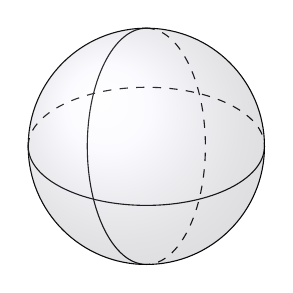
\begin{tikzpicture}[scale=1.5]
    \draw (-1,0) arc (180:360:1cm and 0.5cm);
    \draw[dashed] (-1,0) arc (180:0:1cm and 0.5cm);
    \draw (0,1) arc (90:270:0.5cm and 1cm);
    \draw[dashed] (0,1) arc (90:-90:0.5cm and 1cm);
    \draw (0,0) circle (1cm);
    \shade[ball color=blue!10!white,opacity=0.20] (0,0) circle (1cm);
\end{tikzpicture}
\end{center}
Consider a sphere with radius $r$ with metric,
\[ g_{\al\be} = r^2 \mtrx{1 & 0 \\ 0 & \sin^2\te} \]
With general vector on the sphere $x^\mu$ with,
\[ x^\mu = \mtrx{\te \in \bs{0,\pi}\\ \phi\in \bs{0,2\pi}} \]
Therefore the velocity is $V^\mu$,
\[ V^\mu = \mtrx{\dot{\te} \\ \dot{\phi}}\]
Let our curvilinear parameter of the geodesic be $\tau$ and take $\tau$ to be the arclength. By doing so, we enforce that $V^\al V_\al = + 1$. Therefore since the arclength $\dif \tau^2 = x^\al g_{\al\be} x^\be$,
\[ +1 = V^\al g_{\al\be} V^\be = \der{x^\al}{\tau} g_{\al\be} \der{x^\be}{\tau} = \der{\tau^2}{\tau^2} = r^2\dot{\te}^2 + r^2\sin^2 \te \dot{\phi}^2 \]
Therefore the Euclidean metric used gives $V^\al$ to be spacelike.  This normalization condition $V^\al V_\al = 1$ is \textit{very} important. Finally, our geodesic must satisfy the geodesic equation.
\[ \der{}{\tau}V^\al + {\Ga^\al}_{\be\ga} V^\be V^\ga = 0 \]
The Christoffel symbols for this metric are given by ($1 = \te , 2 = \phi$),
\[ {\Ga^2}_{21} = {\Ga^2}_{12} = \f{\cos \te }{\sin \te} \qquad {\Ga^1}_{22} = - \sin \te \cos \te \]
Only three terms of the $2^3 = 8$ Christoffel symbols are non-zero. The Geodesic equation becomes,
\[ \ddot{\te} + {\Ga^{1}}_{\be\ga} V^\be V^\al = 0 \implies \ddot{\te} - \sin \te \cos \te \dot{\phi}\dot{\phi} = 0 \eq \label{eq:sphere1}\]
\[ \ddot{\phi} + {\Ga^{2}}_{\be\ga} V^\be V^\al = 0 \implies \ddot{\phi} + 2\f{\cos \te}{\sin \te}\dot{\te}\dot{\phi} = 0 \eq \label{eq:sphere2} \]
Noting the very important factor of $2$. We can now solve these coupled second order ODEs. First take the case of $\dot{\phi} = 0$ or that $\phi$ is constant. \eqref{eq:sphere1} gives $\te = a \tau + b$. The normalization condition implies that $a = \pm\f{1}{r}$ in this case of $\dot{\phi} = 0$. This correspond to slices through the sphere at fixed phi. This is a \textbf{great circle} or by analogy on the surface of the earth, these are meridians. \\

Let use examine the other case of $\te$ being constant. In this case, \eqref{eq:sphere2} indicates that $\ddot{\phi}= 0 \implies \phi = d \tau + e$. Also \eqref{eq:sphere1} gives,
\[ -\sin\te \cos\te \br{\dot{\phi}}^2 = 0 \implies \dot{\phi}^2 = 0  \text{ or } \sin\te\cos\te = 0 \]
Note that if $\dot{\phi}^2 = 0$, this forces $d=0$ which violates the normalization condition. It also corresponds to a fixed point. Alternatively, $\sin\te\cos\te = 0$ suggests $\te = \pi / 2 + n\pi$. Note that $\sin \te \neq 0, \pi$ since this makes \eqref{eq:sphere2} singular. This solution corresponds to the equator of the sphere. The set of all solutions are all of the great circles on the sphere.

\subsubsection{Geodesics \& Path Length}

When dealing with the Euclidean metric, the geodesics are the straight lines or equivalently the \textbf{shortest path}.
\[ \text{geodesic} \implies \text{shortest path} \]
However when dealing with the Lorentzian metric, time like geodesics are the \textbf{longest path}.
\[ \text{geodesic} \implies \text{longest path} \]
This is to be expected because light-like vectors have a minimum arclength of $0$. Therefore in order to make the action of the path have zero variation $\de S = 0$, the extremized path is one with maximum action $S$.

\subsection{Curvature}

Curvature can be examined as a rotation of vectors that are parallel transported around a loop.
\begin{center}
\begin{tikzpicture}[
    scale=1.0,
    decoration={post length=0.1mm, pre length=0.1mm, markings, mark=at position 0.5 with {\arrow{>}}}
]
    \draw[postaction={decorate}, thick] (0,0) -- (1,2);
    \draw[postaction={decorate}, thick] (1,2) -- (3,2);
    \draw[postaction={decorate}, thick] (3,2) -- (2,0);
    \draw[postaction={decorate}, thick] (2,0) -- (0,0);
    \draw[->, thick, blue] (1,2) -- (0.7, 2.3);
    \node[blue, above left] (lx) at (0, 0.5) {$x_i = x_f$};
    \draw[->, thick, blue] (3,2) -- (2.7, 2.3);
    \draw[->, thick, blue] (2,0) -- (1.7, 0.3);
    \draw[->, thick, blue] (0,0) -- (-0.3, 0.3);
\end{tikzpicture}
\end{center}

When moving around the loop the vector $x^\mu$ is not modified.
\[ x^\mu_i = x^\mu_f \implies \text{ no curvature} \]

Where as for the case of a loop on a sphere the vectors do not match,
\[ x^\mu_i \neq x^\mu_f \implies \text{ curvature} \]

\textbf{Definition}: Using $\del_\mu$ as the Levi-Civita connection, the \textit{Riemann Curvature Tensor} is defined by,
\[ \br{\del_\mu \del_\nu - \del_\nu \del_\mu} V^\al = {{R_{\mu\nu}}^\al}_\be V^\be \]
This tensor ${{R_{\mu\nu}}^\al}_\be$ encodes the curvature. Expressed in terms of the Christoffel symbols,
\[ {R^{\rho}}_{\sigma \mu \nu} = \di_\mu {\Ga^\rho}_{\nu\sigma}- \di_\nu {\Ga^\rho}_{\mu\sigma} + {\Ga^\rho}_{\mu\lambda}{\Ga^\lambda}_{\mu\sigma} - {\Ga^\rho}_{\nu\lambda}{\Ga^\lambda}_{\mu\sigma} \]
Notice that when dealing with $4d$ spacetime, the Riemann tensor has $4^4 = 256$ components. It can be viewed as a matrix of matrices. This is a lot of components. Luckily, the symmetries of $\Ga$ reduce the number of unique terms. The symmetries are as follows.
\[ R_{\rho \sigma \mu \nu} = - R_{\sigma \rho \mu \nu} = - R_{\rho \sigma \nu \mu} \note{Antisymmetric} \]
\[ R_{\rho \sigma \mu \nu} = R_{\mu \nu \rho \sigma } \note{Symmetric in Pairs} \]
Also cyclic permutations of the last three indices summed together are zero. This is the \textit{1st Bianchi identity}
\[ R_{\rho \sigma \mu \nu} + R_{\rho  \mu \nu\sigma} + R_{\rho  \nu\sigma \mu} = 0 \]
The \textit{2nd Bianchi identity} deals with cyclic permutations in the first three indices (including $\del_\mu$),
\[ \del_\lambda R_{\rho \sigma \mu \nu} + \del_\rho R_{ \sigma\lambda \mu \nu} + \del_\sigma R_{\lambda\rho  \mu \nu} = 0 \]
The combination of all of these symmetries reduces the number of components from $256$ to only $20$ independent components.

\section{Einstein Field Equations}

In the previous section we defined the notion of curvature, $R_{\al\be\nu\mu}$ which is a function of $\br{\di \Ga , \Ga}$. Also, the Christoffel symbols are a function of $\br{\di g, g}$. We are looking for a generalization of $\vF_g = m_I \va$. Our analysis of $\De \phi = 4 \pi G \rho$ lead to the suggestion that $g_{\mu\nu}\br{\phi}$; the metric was dependent on $\phi$.

\subsection{Motivation}

Let us take Poisson's equation to get,
\[ \De \phi = 4 \pi G \rho\]
The constants $4 \pi G$ will be generalized to constants $k$, and $\rho$ generalizes to the stress energy tensor $T_{\al\be}$. How does $\De \phi$ modify?
\[ f\br{R_{\al\be\mu\nu}} \stackrel{?}{=} k T_{\al\be} \]
The RHS of this equation is a rank $(0,2)$ tensor. Therefore we will need to contract some of the indices of $R_{\al\be\mu\nu}$. Note that we can not just multiply it by the metric because as a consequence of symmetry,
\[ g^{\al\be} R_{\al\be \mu\nu} = 0 \qquad g^{\mu\nu} R_{\al\be \mu\nu} = 0 \]
Therefore we will contract against the first indices of each pair,
\[ g^{\al\mu} R_{\al\be \mu\nu} \defined R_{\be\nu}\]
This is known as the \textbf{Ricci tensor}. Note that by extension of properties of the curvature,
\[ R_{\be\nu}= R_{\nu\be} \]
Thus Einstein's first proposal is,
\[ R_{\be\nu} = k T_{\be\nu} \]
This is well motivated as both the right and left hand sides are symmetric. However since the stress energy tensor is conserved,
\[ \del^\nu T_{\be\nu} = 0 \]
But we have that,
\[ \del^\nu R_{\be\nu} = \f12 \del_\be R \]
Where $R = R_{\al\be} g^{\al\be}$ is known as the \textbf{Ricci scalar}. Therefore this first proposal is not consistent.\\

How can we modify this to maintain consistency? Define a new quantity,
\[ G_{\be\nu} = R_{\be\nu} - \f12 R g_{\be\nu} \]
Such that it is divergenceless.
\begin{align*}
\del^\nu G_{\be\nu} &= \del^\nu R_{\be\nu} - \f12 \del^\nu \br{R g_{\be\nu}}\\
&= \del^\nu R_{\be\nu} - \f12 R\del^\nu  g_{\be\nu}\\
&= \del^\nu R_{\be\nu} - \f12 R\del_\be \\
&= \f12 \del_\be R - \f12 R\del_\be \\
&= 0 \\
\end{align*}
However, is this $G$ unique? Obviously we can add any constants that are compatible with the metric. Therefore introduce the \textbf{cosmological constant} $\Lambda$.
\[ G_{\be\nu} = R_{\be\nu} - \f12 R g_{\be\nu}  + \Lambda g_{\be\nu}\]
Therefore we have $G_{\be\nu} = G_{\nu\be}$ and that $\del^\nu G_{\be\nu} = 0$. Therefore,
\[ G_{\be\nu} = k T_{\be\vu} \]
Where $k$ is yet to be determined.\\

To determine what $k$ is, we should be able to recover Newton's law of gravity in a non-relativistic limit. Consider a weak field stationary metric.
\[ g_{\al\be} = \eta_{\al\be} + h_{\al\be} = \eta_{\al\be} -2 \phi\de_{\al\be}\]
Where $\pder{}{x^\be} h_{\al\be} = 0$. Now we can calculate $T_{\al\be}$. Consider a perfect fluid as a dust with pressure $P= 0$ and mass density $\rho=0$.
\[ T^{\al\be} = \rho V^\al V^\be \]
For $h_{\al\be} \ll 1$ or in a weak gravitational field, a little bit of work yields,
\[ R_{\al\be} = -\f12 \Box h_{\al\be} \]
In the limit that $c \gg 1$ we obtain that the D'Alembertian becomes the Laplacian.
\[ R_{\al\be} = \De \phi \de_{\al\be} \]
Therefore we obtain (assuming $\Lambda = 0$ since we are dealing with Newtonian physics),
\[ G_{\al\be} = k T_{\al\be} \]
\[ R_{\al\be} - \f12 R g_{\al\be} = k T_{\al\be} \eq \label{eq:eineqn}\]
Now we take the trace of this equation.
\[ R - \f12 R g_{\al\be} g^{\al\be} = k T_{\al\be}g^{\al\be} \]
Notice that $g_{\al\be} g^{\al\be} = 4$, since we are in a 4 dimensional spacetime.
\[ g^{\al\be} g_{\be\ga} = {\de^\al}_{\ga} \]
If we explicitly sum up this product,
\[ g^{\al\be} g_{\be\al} = {\de^\al}_{\al} \]
We obtain the \textit{trace} of the identity matrix which yields $4$.
\[ -R = k T_{\al\be}g^{\al\be} = kT \]
Therefore we can write \eqref{eq:eineqn} as,
\[ R_{\al\be} = k T_{\al\be} + \f12 R g_{\al\be} \]
\[ R_{\al\be} = k T_{\al\be} - \f12 k T g_{\al\be} \]
Switching to the rest frame of the fluid, we obtain $T_{\al\be} = \rho V^\al V^\be$ as,
\[ T_{\al\be} = \mtrx{\rho & 0 & 0 & 0 \\0 & 0 & 0 & 0 \\0 & 0 & 0 & 0 \\0 & 0 & 0 & 0} \]
The only remaining component is $T_{00} = \rho$.
\[ R_{00} = k T_{00} - \f12 k T_{00} g^{00} g_{00}\]
Notice that $g^{00}g_{00}$ is given by,
\[ g_{00} = -1 - 2 \phi \qquad g^{00} = -1 + 2 \phi \]
\[ g^{00}g_{00} = 1 + O\br{\phi^2} \approx 1 \]
Therefore,
\[ R_{00} = \f12 k T_{00} = \f12 k \rho \]
\[ +\De \phi = \f12 k \rho \]
Which restricts $k$ to be $k = 8 \pi G$. Finally we obtain,
\[ G_{\al\be} = R_{\al\be} - \f12 R g_{\al\be} + \Lambda g_{\al\be} = 8 \pi G T_{\al\be} \]
This is \textbf{Einstein's field equation}. This acts as our generalization of $\De \phi = 4 \pi G \rho$.
\end{document}
